\documentclass[output=paper]{langscibook}
\ChapterDOI{10.5281/zenodo.15148174}
\author{H. Ekkehard Wolff\orcid{}\affiliation{Universität Leipzig}}
\title[Typology and evolution of minimal vowel systems in Central Chadic ]{Typology and evolution of minimal vowel systems in Central Chadic (Afroasiatic)}
\abstract{The chapter summarises arguments and presents selected data in support of the reconstruction of a minimal vowel system *a, *ə for the proto-language of the Central branch of the Chadic language family within the Afroasiatic phylum.  In this system, */a/ is the only vowel phoneme and *ə is a non-phonemic ``intrusive'' vowel. *i and *u occur in phonetic surface realisations representing not separate phonemes but conditioned allophones of the approximants *j and *w.

Certain reconstructed segments may ``prosodise'' by dissociating from articulatory features, which turn into ``floating'' suprasegmental features (= ``prosodies'') that re-associate with other segments within the word. Thereby, labialisation and palatalisation create, by raising, fronting and back-rounding, prosody-induced ``col\-ourings'' of other segments. These diachronic processes yield a plethora of phonetic surface realisations of vowels and (new) series of palatalised and labialised (but also prenasalised and glottalised) consonants in the modern languages, quite a few of which are characterised by very rich surface consonant inventories and multi-vowel systems.

The chapter discusses the evolution of the minimal vowel system in Proto-Central Chadic in cross-linguistic typological perspective and points out potential implications for the reconstruction of Proto-Afroasiatic. The chapter tentatively proposes a speculative hypothesis according to which the ultimate common proto-language may have been completely ``vowelless''.

\keywords{minimal vowel system,  Afroasiatic, Central Chadic, historical phonology, typology }
}
\IfFileExists{../localcommands.tex}{
  \addbibresource{../localbibliography.bib}
  \usepackage{tabularx, multicol, multirow, longtable}
\usepackage{url}
\urlstyle{same}

\usepackage{orcidlink}
\definecolor{orcidlogocol}{cmyk}{0,0,0,1}
\RenewDocumentCommand{\LinkToORCIDinAffiliations}{ +m }
  {%
    \orcidlink{#1}\,%
  }
\SetupAffiliations{orcid placement=before}

\usepackage{siunitx}
\sisetup{detect-weight=true, detect-family=true, group-digits=none}

\usepackage{mathtools}
\usepackage{langsci-optional}
\usepackage{langsci-lgr}
\usepackage{langsci-gb4e}

\usepackage{stmaryrd}
\usepackage[capitalize]{cleveref}
\babelfont[macedonian]{rm}[Language=Macedonian,ItalicFont=LibertinusSerif-Italic.otf]{LibertinusSerif-Regular.otf}
\usepackage{eqparbox}
\usepackage[autostyle]{csquotes}
\usepackage[linguistics]{forest}

\usetikzlibrary{positioning, matrix}
\usepackage[glosses,inline]{leipzig}
\PassOptionsToPackage{xindy,toc,nopostdot}{glossaries}
\usepackage{glossary-inline}
\setglossarystyle{inline}
\makeglossaries

\usepackage{phonrule}
\usepackage{threeparttable}


\usepackage{textcomp,gensymb}


\usepackage[preservefont]{tipauni}

\usepackage[normalem]{ulem}

\usepackage{enumitem} %so lists aren't ugly
	
\usepackage{threeparttable}	%allows tables with tablenotes. note marks: †‡
	\makeatletter 
	\g@addto@macro\TPT@defaults{\footnotesize} 
	\makeatother

\usepackage{colortbl}
	\definecolor{Pink}{rgb}{0.96, 0.76, 0.76} 
	\definecolor{PaleBlue}{rgb}{0.67, 0.9, 0.93}
	\definecolor{carolinablue}{rgb}{0.6, 0.73, 0.89}
	\definecolor{goldenyellow}{rgb}{1.0, 0.87, 0.0}
	\definecolor{Orange}{rgb}{1.0, 0.66, 0.07}
	\definecolor{puce}{rgb}{0.8, 0.53, 0.6}
	\definecolor{turquoisegreen}{rgb}{0.63, 0.84, 0.71}


% add all extra packages you need to load to this file
\usepackage{langsci-textipa}
\usepackage{vowel}
\usepackage{textgreek}

% \usepackage{langsci-branding}
% \usepackage{subcaption}
\usepackage{subfigure}

\usepackage{tabto}


\usetikzlibrary{tikzmark}
\usepackage{pgfplots}


\newfontfamily\tibetan{NotoSerifTibetan-Regular.ttf}
\usepackage{langsci-branding}
\usepackage{hyphenat}

\usepackage{accents}

  \renewcommand{\lsChapterFooterSize}{\footnotesize}

\makeatletter
\let\thetitle\@title
\let\theauthor\@author
\makeatother

\newcommand{\togglepaper}[1][0]{
   \bibliography{../localbibliography}
   \papernote{\scriptsize\normalfont
     \theauthor.
     \titleTemp.
     To appear in:
     Natalia Kuznetsova, Cormac Anderson \& Shelece Easterday (ed.).
     Rarities in phonetics and phonology.tex.
     Berlin: Language Science Press. [preliminary page numbering]
   }
   \pagenumbering{roman}
   \setcounter{chapter}{#1}
   \addtocounter{chapter}{-1}
}

\newbool{bookcompile}
\booltrue{bookcompile}
\newcommand{\bookorchapter}[2]{\ifbool{bookcompile}{#1}{#2}}

\newcommand{\textarab}[1]{\RL{\arabicfont #1}}

\newcommand\mb[1]{\eqparbox[t]{examples}{#1}\hspace{1em}}
\newcommand\mbi[1]{\mb{#1}}
\newcommand{\twe}[3]{\mbi{#1}\eqparbox[t]{orths}{\emph{#2}}\hspace{1em}`#3'\hspace{1em}} % three-way example
\providecommand\glottocode[1]{[\href{https://glottolog.org/resource/languoid/id/#1}{#1}]}
\newcommand{\phonreal}[1]{\ensuremath{\llbracket}#1\ensuremath{\rrbracket}}

\DeclareRobustCommand\dash{\unskip\nobreak\thinspace\textendash\allowbreak\thinspace\ignorespaces}

\forestset{minus/.style={edge label={node[midway, left] {\ensuremath{-}\hspace*{2mm}}}},
plus/.style={edge label={node[midway, right] {\hspace*{2mm}\ensuremath{+}}}}}
\providecommand\ipa[1]{#1}


\newcommand{\tone}[1]{\textsuperscript{#1}}

\newcommand{\orthog}[1]{\textit{#1}}
\newcommand{\gloss}[1]{`#1'}

\newcommand{\glottolog}[1]{\texttt{\href{https://glottolog.org/resource/languoid/id/#1}{#1}}}

\newcolumntype{O}{>{\itshape }l<{}}
\newcolumntype{G}{>{`}l<{'}}

\newcounter{tabsubcounter}
\newcommand{\tablecounter}{\setcounter{tabsubcounter}{0}}
\newcommand{\TC}{\stepcounter{tabsubcounter}\alph{tabsubcounter}.}

\usetikzlibrary{chains,positioning,calc,decorations.markings}
\tikzset{
	seg/.style={text height=0.6em, text depth=0.3em},
	moraic-structure/.style={xscale=0.6,yscale=1.1, text height=0.65em,text depth=0.25em},
 }

%05_Culhane_Edwards
%%%%%%%%%%%%%%%%%%%%%%%%%%%%%%%%
%%	Symbols and Characters  	%%
%%%%%%%%%%%%%%%%%%%%%%%%%%%%%%%% αβσµ

\newcommand{\tl}{\char`~}						%middle tilde ~
\renewcommand{\Q}{\textquotesingle}		%straight apostrophe444
\newcommand{\ra}{→} 								%right arrow ->
\newcommand{\0}{∅} 									%zero symbol
\newcommand{\gap}{\textunderscore} 	%underscore
%\renewcommand{\j}{ʤ}								%dezh digraph
\newcommand{\syll}{σ}								%lowercase sigma medial form
\newcommand{\wrd}{ω}								%lowercase omega
\newcommand{\ft}{φ}									%lowercase phi
\newcommand{\gw}{gʷ}								%g with superscript w
\newcommand{\B}{β}									%voiced bilabial fricative
\newcommand{\hp}{\hphantom}					%space equal to width of argument
\newcommand{\it}{\textit}	%italics

%%%%%%%%%%%%%%%%%%%%%%%%%%%%%%%%
%%	Font Styles & Formatting	%%
%%%%%%%%%%%%%%%%%%%%%%%%%%%%%%%%

\definecolor{DarkBlue}{RGB}{0,0,130}										%dark blue colour
% \newcommand{\ve}[1]{\textcolor{DarkBlue}{\textit{#1}}}	%vernacular text
\newcommand{\ve}[1]{{\textit{#1}}}	%vernacular text
\definecolor{DarkRed}{RGB}{150,0,0}											%dark red colour
% \newcommand{\tbr}[1]{\textcolor{DarkRed}{\textbf{#1}}}	%Bold red text
\newcommand{\tbr}[1]{{\textbf{#1}}}	%Bold red text
%\renewcommand{\it}{\textit}																%italics
\newcommand{\tsc}{\textsc}															%small caps
\newcommand{\sub}{\textsubscript}												%subscript
\newcommand{\su}{\textsuperscript}											%superscript

%%%%%%%%%%%%%%%%%%%%%%%%%%%%%%%%%%%%%%%%%%%%%%%%%%%%
%% Tables %% Tables %% Tables %% Tables %% Tables %%
%%%%%%%%%%%%%%%%%%%%%%%%%%%%%%%%%%%%%%%%%%%%%%%%%%%%

% \newcommand{\mc}{\multicolumn}									%multicolumn
% \newcommand{\st}[1]{\setlength{\tabcolsep}{#1}}	%reduce column width in tables
%
%%%%%%%%%%%%%%%%%%%%%%%%%%%%%%%%
%%    Cross   References      %%
%%%%%%%%%%%%%%%%%%%%%%%%%%%%%%%%

% \def\Plus{\texttt{+}}
% \def\Minus{\texttt{-}}
% \newcommand{\GS}{ʔ}
% \def\SH{ʃ}
% \newcommand{\TSH}{ʧ}
% \def\ZH{ʒ}
% \def\DZH{ʤ}
% \def\:{ː}
% \def\UP{\textsuperscript}
% \def\rs{ʂ}
% \newcommand{\rn}{ɳ}
% \def\rt{ʈ}
% \def\tllr{ɺ}
% \newcommand{\Bb}{β}
% \def\Eps{ɛ}
% \def\Oo{ɔ}
% \def\Gm{ɣ}
% \def\NG{ŋ}
% \def\barU{ʉ}
\newcommand{\CM}{\ding{51}}
\newcommand{\XM}{\ding{53}}
% \newcommand{\tap}{ɾ}
% \def\darkL{ɫ}
% \def\schwa{ə}
%
% \def\BUL{\textbullet}


%%%%%%%%%%%%%%
%					%
%	Secondaries		%
%					%
%%%%%%%%%%%%%%
%	Post
\newcommand{\Post}[2]{#1\textsuperscript{#2}}
%	Pre
\newcommand{\Pre} [2] {\textsuperscript{#1}#2}
%	Undertilde
\newcommand{\utilde}[1]{\ensuremath{\smash{\underset{\mathclap{\sim}}{\text{#1}}}}}
%	Devoiced
% \newcommand{\VCLS}[1]{\textsubring{#1}}
%%%%%%%%%%%
%				%
%	Definitions		%
%	Markup		%
%				%
%%%%%%%%%%%
% \def\->{$\rightarrow$}
% \def\__{\underline{\hspace{1em}}}
\def\NoPoss{\cellcolor{gray!30}}

\newcommand{\VOICELESS}{\textsc{voiceless}}
\newcommand{\VOICED}{\textsc{voiced}}
\newcommand{\tablenote}[2][1]{\parbox{#1\textwidth}{\footnotesize\raggedright #2}}

\newcommand{\appref}[1]{Appendix~\ref{#1}}
\renewcommand{\sectref}[1]{Section~\ref{#1}}


\newcommand{\dobuibox}[5]{#1\\[-1.1em]
\hspace*{-.8cm}
 \begin{tabularx}{.9\textwidth}{@{}lQQ@{}}
       &  {oral} &  {nasal} \\
       \midrule
     {controlled} &\parbox[t]{4cm}{\raggedright  #2} & \parbox[t]{4cm}{\raggedright #3} \\
     \tablevspace
     {ballistic} &\parbox[t]{4cm}{\raggedright  #4} & \parbox[t]{4cm}{\raggedright  #5} \\
 \end{tabularx}
}

\newfontfamily\VdottildeFont{LibertinusVdottilde.otf}

\newcommand{\Vdottilde}{{\VdottildeFont V̰̣}}

% \renewcommand{\keywords}[1]{\textbf{#1}}
 
  %% hyphenation points for line breaks
%% Normally, automatic hyphenation in LaTeX is very good
%% If a word is mis-hyphenated, add it to this file
%%
%% add information to TeX file before \begin{document} with:
%% %% hyphenation points for line breaks
%% Normally, automatic hyphenation in LaTeX is very good
%% If a word is mis-hyphenated, add it to this file
%%
%% add information to TeX file before \begin{document} with:
%% %% hyphenation points for line breaks
%% Normally, automatic hyphenation in LaTeX is very good
%% If a word is mis-hyphenated, add it to this file
%%
%% add information to TeX file before \begin{document} with:
%% \include{localhyphenation}
\hyphenation{
    af-fri-cates
    al-ve-o-pal-a-tal
    Ama-nu-ban
    Ara-wak-an
    Árna-son
    Ber-ber
    can-di-dates
    Cam-er-oon
    Chi-nan-tec
    Chir-ko-va
    Crai-o-ve-a-nu
    di-chot-o-my
    Ec-ua-do-rian
    Ec-ua-dor
    elec-tro-glot-to-gra-phy
    Faro-ese
    Ike-ma
    Kuznet-sova
    Mes-kwa-ki
    Mio-ma-fo
    mono-mor-aic
    Ne-ca-xa
    Oto-man-gue-an
    par-a-digm
    post-as-pi-rat-ed
    post-as-pi-ra-tion
    pre-as-pi-rat-ed
    pre-as-pi-ra-tion
    pros-o-dic
    pros-o-dies
    re-con-struc-table
    Sheh-ret
    Svan-tes-son
    Ta-ras-can
    Tórs-havn
    Ural-ic
    epen-the-sis
    Anin-dil-yak-wa
    Mi-nyag
    Na-ka-ma
}

\hyphenation{
    af-fri-cates
    al-ve-o-pal-a-tal
    Ama-nu-ban
    Ara-wak-an
    Árna-son
    Ber-ber
    can-di-dates
    Cam-er-oon
    Chi-nan-tec
    Chir-ko-va
    Crai-o-ve-a-nu
    di-chot-o-my
    Ec-ua-do-rian
    Ec-ua-dor
    elec-tro-glot-to-gra-phy
    Faro-ese
    Ike-ma
    Kuznet-sova
    Mes-kwa-ki
    Mio-ma-fo
    mono-mor-aic
    Ne-ca-xa
    Oto-man-gue-an
    par-a-digm
    post-as-pi-rat-ed
    post-as-pi-ra-tion
    pre-as-pi-rat-ed
    pre-as-pi-ra-tion
    pros-o-dic
    pros-o-dies
    re-con-struc-table
    Sheh-ret
    Svan-tes-son
    Ta-ras-can
    Tórs-havn
    Ural-ic
    epen-the-sis
    Anin-dil-yak-wa
    Mi-nyag
    Na-ka-ma
}

\hyphenation{
    af-fri-cates
    al-ve-o-pal-a-tal
    Ama-nu-ban
    Ara-wak-an
    Árna-son
    Ber-ber
    can-di-dates
    Cam-er-oon
    Chi-nan-tec
    Chir-ko-va
    Crai-o-ve-a-nu
    di-chot-o-my
    Ec-ua-do-rian
    Ec-ua-dor
    elec-tro-glot-to-gra-phy
    Faro-ese
    Ike-ma
    Kuznet-sova
    Mes-kwa-ki
    Mio-ma-fo
    mono-mor-aic
    Ne-ca-xa
    Oto-man-gue-an
    par-a-digm
    post-as-pi-rat-ed
    post-as-pi-ra-tion
    pre-as-pi-rat-ed
    pre-as-pi-ra-tion
    pros-o-dic
    pros-o-dies
    re-con-struc-table
    Sheh-ret
    Svan-tes-son
    Ta-ras-can
    Tórs-havn
    Ural-ic
    epen-the-sis
    Anin-dil-yak-wa
    Mi-nyag
    Na-ka-ma
}
 
  \togglepaper[7]%%chapternumber
}{}

\begin{document}
\maketitle 
%\shorttitlerunninghead{}%%use this for an abridged title in the page headers
% ATTENTION: Diacritics on the following phonetic characters might have been lost during conversion: {'ʊ', 'ɨ', 'ɔ', 'ɛ', 'ə', 'ɪ', 'ʉ'}

\section{Introduction}
\label{sec:Wolff:1}
\subsection{Aims and focus}
\label{sec:Wolff:1.1}

This paper focuses on typological and historical insights gained from the internal and comparative reconstruction of vowel systems in the languages of the Central (also referred to as ``Biu-Mandara'') branch of the Chadic language family in West and Central Africa. Until quite recently, vowels in Chadic languages were considered to be nearly impossible to reconstruct by the application of a classic comparative method under the Neogrammarian Hypothesis, because of an apparent absence of regular sound correspondences of vowels between pairs of languages. In the available literature (e.g. \citealt{Newman1977, Newman2006, JungraithmayrShimizu1981, Stolbova2016, Wolff2017}), therefore, there is hitherto no consensus on the number, quality, and distribution of contrastive vowels with regard to lexical reconstructions for common Proto-Chadic (PC) or even those for individual branches of the family, such as Proto-Central Chadic (PCC). Severe analytical problems result from the fact that present-day Chadic languages are synchronically described as possessing any number between one (always \mbox{/a/}) and 17 short and long oral vowels \citep{Wolff2017}. So far, no overarching theoretical and typological account has been proposed that would provide a coherent relationship between the highly different synchronic vowel systems that one finds in Chadic languages, not to mention a satisfactory historical account of how these various synchronic systems have developed from a common proto-language. This deplorable lack of solid lexical comparisons and reconstructions from Chadic continues to have negative effects also on the reconstruction of the deepest proto-language, Proto-Afroasiatic (PAA), which is genetically ancestral to Chadic (\citealt{Greenberg1963, Newman1980}).

\begin{sloppypar}
The paper explores and summarises the diachronic hypotheses which allow the reconstruction of a historical scenario of vocalogenesis. According to this scenario, the common proto-language (PC) was characterised by a minimal vowel system. This system then historically underwent various processes of phonologisation of (i) allophones of segmental phonemes, and (ii) variants of an almost fully predictable pro- and epenthetic vowel schwa. The synchronic reflexes in modern Chadic languages are multi-vowel systems. Some modern languages, however, have retained variants of the original minimal vowel system. The proposed historical scenario of vocalogenesis would explain the considerable typological variation of vowel systems in modern Chadic languages, which has hitherto intrigued and frustrated researchers.
\end{sloppypar}

After addressing the central notion of a minimal vowel system (\sectref{sec:Wolff:1.2}), the paper briefly introduces the Central Chadic languages (\sectref{sec:Wolff:1.3}). It then sketches out a number of non-trivial characteristics of Central Chadic phonology and introduces a non-canonical (“prosodic”) methodological approach to Chadic phonology, which is argued to best capture both synchronic and diachronic features of this language family (\sectref{sec:Wolff:1.4}). The introductory section closes with a short illustration of a multi-tiered approach to Central Chadic phonology (\sectref{sec:Wolff:1.5}).

In \sectref{sec:Wolff:2}, the paper focuses on the vocalic domain in Central Chadic languages and its segmental and salient suprasegmental (“prosodic”) units. This section aims to show why and how a non-canonical prosody-based approach allows relevant generalisations concerning the underlying phonological system that are missed by non-prosodic approaches. 

In \sectref{sec:Wolff:3}, the paper embeds the results and insights gained from the prosody-based phonological analysis of the vocalic domain in Central Chadic within a global cross-linguistic typological survey of minimal vowel systems. The section ends with an outlook on the implications for historical typology of Afroasiatic vowel systems and suggests directions for further typological and comparative research.

\sectref{sec:Wolff:4} presents a short summary.

\subsection{Minimal vowel systems as ``rarities'' in cross-linguistic perspective}
\label{sec:Wolff:1.2}

Since early works by Trubetzkoy (\citeyear{Trubetzkoy1925, Trubetzkoy1939}) on vowel systems, as well as those by \citet{Jakovlev1923} and particularly \citet{Kuipers1960} on Northwest Caucasian Kabardian, so-called minimal vowel systems have received controversial interpretations in phonological theory. They might be considered phonological rarities. While all natural human languages would appear to possess vowels in phonetic surface realisations, this is arguably not so on increasingly abstract levels of phonological representation. In the presence of only one or no phonemic vowels at all in individual languages and language groups, the notion of vowel system as such and the universal existence of vowel systems in human languages becomes disputable. One-vowel and no-vowel phonological inventories for individual languages and language groups have been postulated cross-linguistically in the past (see \sectref{sec:Wolff:3}), but have almost automatically provoked doubt and alternative proposals; see \citet[59--117]{Anderson2016} for a survey of literature on minimal vowel systems in typological perspective.\footnote{The author acknowledges valuable comments by Cormac Anderson, one of the editors of the present volume, on an early version of this paper.}

Minimal vowel systems have been described for individual languages or small groups of languages in diverse parts of the world (for details and sources see \sectref{sec:Wolff:3}): Northwest Caucasian (Kabardian, Abkhaz, Ubykh); Goidelic (Modern Irish); languages of Papua New Guinea (Sepik-Ramu: Ndu; Nor-Pondo: Yimas; Piawi: Haruai); Marshallese; Chinese languages (including Mandarin); Upland Yuman (Walapai); Salishan (Nuxálk/Bella Coola); Arandic languages; Anindilyakwa; Berber/Amazigh (Tashelhiyt); Chadic (Central Chadic). The present chapter focuses on Central Chadic languages, which together with distantly related Tashelhiyt (Berber/Amazigh) within Afroasiatic, represent the African continent in this survey.

Central to a typological approach to minimal-vowel systems is the recognition of a special phonological status of two approximants, */j/ and */w/, and their relation to high vowels [i] and [u].\footnote{Note that in established practice for African including Chadic languages, IPA /j/ is usually rendered by the graphic symbol /y/. I will follow this established usage in the body of this paper.} The essential structural ambivalence (indicated by the feature specification [±syll]) of these approximants has earned them the labels ``semi-vowels'' and ``semi-consonants'' in traditional phonological literature; Semitic scholarship speaks of ``weak radicals''. This ambivalence, which some authors consider to essentially dissolve the distinction between vowels and consonants, motivates a review of the vocalic space in languages. For my historical reanalysis of Central Chadic languages, IPA *j and *i on the one hand, and *w and *u on the other, are not different phonemes, but rather conditioned allophones of each other in perfect complementary distribution. This raises the ontological question as to the phonological status of vowels and consonants. It is revealing that by reference to \citet{ManasterRamerBicknell1995}, \citet[112]{Anderson2016} reports:

\begin{quote}\relax
There is nothing at all odd about a language with the vowel system /i a u/, with a CVCV syllable structure, and with distinct semivowels /j w/, the authors argue, but if these features are combined, then the vowels /i u/ and the semivowels /j w/ will always be in complementary distribution, and the difference between them cannot be considered phonemic. That being the case, it makes no difference in most versions of phoneme theory, whether one writes /j/ and /w/, or /i/ and /u/, but it is inconsistent to do both.
\end{quote}

In the context of discussing Mandarin Chinese, \citet[71]{Anderson2016} further references \citet[75]{Hockett1955} by saying that “[i]n his own terminology, /i/ and /u/ are not strictly speaking vowels, given the fact that they can occur both as syllable peak and syllable margin”. Note also that in his seminal analysis of \textit{Die Silbenauslautgesetze des Hausa} [The laws pertaining to syllable coda in Hausa],\footnote{Known as ``Klingenheben's Law''; for an English translation see \citet{Newman2004}.}  a West Chadic language, \citet{Klingenheben1927} made it a point to transcribe conventional /y/ and /w/ in Hausa as vowels /i̯/ and /u̯/ and explicitly stated his motivation for doing so.

This particular view on the relationship between the approximants IPA /j, w/ and the high vowels [i, u] is central to the present paper (\sectref{sec:Wolff:2.3}). It further links a proposed analysis to the diachronic hypothesis about an underlying ``vowelless'' system (see \sectref{sec:Wolff:3}):

\begin{quote}\relax
Given the existence of vowelless analyses of a number of languages […] it is unclear if the existence of a distinct class of vowels is a phonological universal at all. If these analyses are omitted from consideration, then it would indeed be possible to state an absolute universal for the world’s vowel systems: all languages have /a/ \citep[102]{Anderson2016}.\footnote{This would be at variance with \citegen{Comrie1991} description of Haruai, who prefers to transcribe the single phonemic vowel as /ə/ \citep[102]{Anderson2016}. The exact phonetic identification of such basic central vowels, whether [ɐ, ɨ] or [a, ə] is of no concern here; the established convention in Chadic linguistics is the graphic representation <a, ə>.}
\end{quote}

This generalisation by Anderson is supported by the author’s research on Central Chadic languages, as reported in the present paper. It will be shown that, if one assumes an underlying minimal vowel system, the latter can be based on one vowel phoneme only, which must be */a/. If the description is based on a two-vowel system, this will be a vertical system in which the phonemic vowels are \mbox{*/a/} ([+low, -high]) and \mbox{*/ə/} ([-low, -high]). Given the role that the approximants \mbox{/j/} and \mbox{/w/} play in forming ``purely consonantal'' roots in Chadic and generally in Afroasiatic languages, they are best grouped together with the consonants rather than with the vowels. Structurally, therefore, surface \mbox{[i]} and \mbox{[u]} do not count as manifestations of vowel phonemes, which leaves \mbox{*a} and \mbox{*ə} as basic vowels in a minimal vertical vowel system.

\subsection{Central Chadic languages}
\label{sec:Wolff:1.3}
Central Chadic languages form one of four branches of the Chadic family. Within the Afroasiatic language phylum, this family is linked to Ancient Egyptian, Berber (Amazigh), Cushitic, Semitic, and possibly the Omotic languages. In a cross\hyp linguistic perspective, Central Chadic would now appear to be the largest known group of languages assumed to share the so-called minimal vowel systems – at least in the diachronic perspective. 

Altogether 196 Chadic languages (according to \citealt{ethnologue24}) are spoken west, south and east of Lake Chad in Central Africa and constitute the largest family within the Afroasiatic language phylum (\citealt{Greenberg1963, Newman1980}). Most of them are under-researched \citep{Newman2006, FrajzyngierShay2012, MeyerWolff2019, WolffPress}. The 79 known Central Chadic (aka Biu-Mandara) languages (\citealt{ethnologue24}) form the largest and most diverse branch within Chadic. 

Chadic languages in general have been notorious for escaping the successful application of the comparative method with regard to vowels (cf. \citealt{Newman1977, JungraithmayrShimizu1981, Stolbova2016}, \citealt{Wolff2017, Wolff2022a}). Within the Chadic family, the languages of the Central Chadic branch, in particular sub-branch A, have long been considered to be phonologically and grammatically the least archaic with regard to retaining typological features from its Afroasiatic genetic heritage. Both views have recently been challenged by the author (\citealt{Wolff2009, Wolff2011, Wolff2017, Wolff2022a, Wolffinpressb}).

\subsection{Some non-trivial (morpho-)phonological features of Central Chadic languages}
\label{sec:Wolff:1.4}

Central Chadic languages are notorious for their typological diversity in terms of their phonological and morphological systems, but they also share a number of non-trivial phonological features, some of which will be considered in this sub-section. 

\subsubsection{A note on data transcription conventions}
\label{sec:Wolff:1.4.1}
A recurrent problem in Chadic typological and comparative linguistics is the absence of standardised transcription conventions and the often unknown linguistic expertise of colonial, missionary, and field linguists, who have compiled and made available primary linguistic data over the last 150 years and more. One finds fairly exact phonetic transcriptions for some language data and rather broad transcriptions for others, which often aim at simultaneously suggesting ``practical'' orthographies for literacy purposes. One finds also transcriptions that are obviously oriented at representing the phonemes of the language. Often the chosen transcription conventions differ from linguist to linguist, occasionally even for the same language. In the absence of phonetically and phonologically reliable transcriptions for many if not most (Central) Chadic languages, one has to make do with the transcriptions found in the available data, including the particular database \citep{Gravina2015} that my most recent work is based on. These original transcriptions of data will always be given in \textit{italics} in this chapter.

In particular the graphic symbols <i, u, e, o> are structurally ambivalent. In broad transcriptions, which are often intended to inform ``practical'' orthographies for hitherto unwritten languages and which are readily available on a typewriter or computer keyboard, <~i, u> in Central Chadic languages may represent:

\begin{itemize}
\item either syllabified conditioned allophones of underlying */y/ and */w/, 
\item or ``coloured'' variants of non-phonemic [ə] (schwa) under Y- and W-pros\-o\-dy effects (see below), which would be the conventionalised transcriptions of phonetically more precise [ɪ] and [ʊ] in the absence of phonological contrasts between /i{\textasciitilde}ɪ/ and /u{\textasciitilde}ʊ/.
\end{itemize}

In turn, <e, o> may represent:

\begin{itemize}
\item either /a/ under Y- and W-prosody effects (see below), which would be the conventionalised transcriptions of phonetically more precise [ɛ] and [ɔ] in the absence of phonological contrasts between /e{\textasciitilde}ɛ/ and /o{\textasciitilde}ɔ/,
\item or a lowered variety of [i, u]) (i.e. syllabified /y, w/) under the appropriate conditions, such as in the neighbourhood to /a/ in an adjacent syllable. 
\end{itemize}

These transcription conventions often blur what is going on both phonetically and phonologically, namely that phonetic [ε] and [ɔ] represent /a/, and [ɪ] and [ʊ] represent schwa, while [e] and [o] often represent lowered /i/ and /u/. Therefore, high vowels in Central Chadic transcriptions are prima facie ambivalent with regard to their phonological status. I argue that only solid phonological and lexical reconstruction will answer to this challenge and, by taking notice of the effects of Y- and W-prosodies, provide unequivocal identification of the respective source segments in the proto-language. For comparative purposes, they need to be assessed from a historical point of view as to whether they are allophones of phonemic */y/ and */w/ or variants of non-phonemic schwa.

Different transcription conventions may also concern graphic representations [ə] and [ɨ] on the one hand, and [ɪ, ɨ] and [ʊ, ʉ] on the other. In most of Chadic linguistic literature, and followed by the author in this chapter, [ə] represents schwa under ∅-prosody (= absence of Y- and W-prosody). While [ə] has become standard transcription of schwa in Chadic linguistics, [ɨ] would be phonetically probably more precise for a number of Chadic languages. Therefore, some authors (including \citealt{Gravina2014,Gravina2015}) prefer to render prosodically ``uncoloured'' schwa as [ɨ]. This is not a trivial issue, since the graphic representation ə (IPA) suggests a central mid vowel, while ɨ (IPA) suggests a central high vowel. For the purpose of this paper and also elsewhere, it is assumed that [ɪ] does and [ɨ] may represent [ə] under Y-prosody, while [ʊ] and [ʉ] represent [ə] under W-prosody.\footnote{The question whether in all or some Chadic languages schwa should be treated as a central mid or rather a high vowel (see \citealt{Roberts2001}) cannot be considered settled. The alternative hypothesis that there were two short central vowels [ə] and [ɨ] as in some Berber languages has never been suggested as likely for Chadic. Rather and more plausibly, Y-prosody can be assumed to either front non-high /ə/ to [ɪ], simply raise it to high [ɨ], or both front and raise it to [i], while W-prosody acts to either round non-high /ə/ to [ʊ] or both raise and round it to [ʉ] and [u]. This would also explain the high degree of overlapping allophones and variants within minimal vowel systems, such as in Central Chadic for */a/: [ɛ{\textasciitilde}a{\textasciitilde}ɔ], for schwa: [ɪ{\textasciitilde}ə{\textasciitilde}ɨ{\textasciitilde}i], [ʊ{\textasciitilde}ə{\textasciitilde}ʉ{\textasciitilde}u], for */y/ (in syllable nucleus): [i{\textasciitilde}e], for */w/ (in syllable nucleus): [u{\textasciitilde}o]. Systematic comparative studies of Chadic vowels have just begun, and such questions as to the high or mid characteristics of ``schwa'' must currently remain subject to further research.} In individual cases and with some sources, however, the interpretation of [ɨ] as raised and non-round (if not slightly fronted) schwa under Y-prosody might involve over-analysis, namely where the source uses [ɨ] to symbolise a true central vowel (under ∅-prosody) that is conventionally labelled ``schwa''.  In case of doubt, the data should be checked against the original source (cf. \citealt{Gravina2015}).

\subsubsection{Root-and-pattern structure}
\label{sec:Wolff:1.4.2}
Recent historical-comparative research (\citealt{Wolff2022a, Wolffinpressb}) has proposed an early and rather basic root-and-pattern structure as important Afroasiatic typological heritage in Central Chadic languages, and probably in Chadic as a whole. This means that reconstructed lexical items in PCC, like in PC and in PAA, consist of a skeleton of consonants (also known as radicals), i.e. a ``root'', in which the approximants */y/ and */w/ count as consonants. This is also why they are called ``weak radicals'' in traditional Semitic scholarship (e.g. \citet{Akesson2001}). The only phonemic vowel */a/ (see \sectref{sec:Wolff:1.4.4}) could be added to these roots in medial interconsonantal positions, which is called the ``pattern''.\footnote{Note that I do not consider the lexical root-final vowel */a/ to be part of the pattern. It is – and debatably so – reconstructed by default for three reasons. (i) When it is present in modern languages, it would need no explanation and it would be clear that one is not dealing with an added grammatical morpheme of sorts. (In earlier reconstructions of African languages, including Chadic, final vowels were almost automatically subtracted from roots and were considered added material, so that ``roots'' would aprioristically end in a consonant. Yet, usually no grammatical function could be identified for such final vowel). (ii) When it is not present in modern languages, which is frequently the case, one would be dealing with apocope/deletion, for which, however, conditioning factors have not yet been identified. (iii) In quite a few instances, one finds schwa in word-final position, which allows two options of analysis: Either one is dealing with a likely conditioned (pre-juncture?) allophone of /a/, or the final /a/ has been deleted and epenthetic schwa has subsequently been inserted. This issue remains open for further research on the level of individual languages and/or language groups.}

Based on the original number of [-syll] segments in the root (radical consonants or radicals), which alone in many Afroasiatic languages carry basic lexical meaning, PCC distinguished several root types. These root types specified whether and how the inter-radical positions were filled by */a/, in addition to the default presence of lexical-final */a/. In these historically underlying root types, I distinguish a-vocalisation from ∅-vocalisation (first suggested in \citealt{Wolff1977}). The basic root types are listed in \tabref{tab:wolff:1}.

\begin{table}
\caption{Basic root types: ∅- and a-vocalisation patterns}
\label{tab:wolff:1}
\begin{tabular}{llll}
\lsptoprule
 & monoradical & biradical & triradical\\
 \midrule
∅-vocalisation & ${\surd}$ Ca & ${\surd}$ C Ca & ${\surd}$ C C Ca\\
a-vocalisation & --- & ${\surd}$ CaCa & ${\surd}$ CaC Ca\\
&  &  & ${\surd}$ C CaCa\\
&  &  & ${\surd}$ CaCaCa\\
\lspbottomrule
\end{tabular}
\end{table}

When these basic root types left open one or more pre- and interconsonantal slots which could potentially be filled by vowels, additional syllabification processes allowed for epenthetic schwa to be inserted. Insertion had followed the lines of a sonority-based hierarchy pertaining to the consonantal environment, until phonotactically acceptable syllable structures were created. The sonority-based hierarchy would appear to be that which is also found to operate in Tashelhiyt (Berber; see \citealt{Kossmann2012}: 28ff. and further below in this chapter): \textit{a} > \textit{i/y}, \textit{u/w} > liquids > nasals > voiced fricatives > voiceless fricatives > voiced stops > voiceless stops. These syllabification processes may have left potential vowel slots unfilled by [ə], because root types did not need to follow a requirement to create simple CV.CV.CV syllable structures; see \tabref{tab:wolff:2}.

\begin{table}
\caption{Synchronically underlying root types showing potential epenthetic vowel insertion. Individual Central Chadic languages may phonetically also require prothetic vowel insertion in cases of word-initial consonant clusters; this is not indicated in the table.}
\label{tab:wolff:2}
\begin{tabular}{llll}
\lsptoprule
 & monoradical & biradical & triradical\\
 \midrule
∅-vocalisation & ${\surd}$ Ca & ${\surd}$ C(ə)Ca & ${\surd}$ C(ə)C(ə)Ca \\
 a-vocalisation &  & ${\surd}$ CaCa & ${\surd}$ CaC(ə)Ca \\
 &  &  & ${\surd}$ C(ə)CaCa\\
 &  &  & ${\surd}$ CaCaCa\\
\lspbottomrule
\end{tabular}
\end{table}

Syllabification in PCC turned the historical root types finally into underlying forms on which the actually occurring surface realisations in modern languages are built. In PCC, consonantal roots underwent multi-step syllabification processes following a sonority-scale hierarchy (see above). At the first step, pre- and interconsonantal positions are filled by */a/ and create first syllable peaks. At the second step, underlying */y/ and */w/, if present in the root, syllabify into their allophones [i] and [u] (\sectref{sec:Wolff:1.4.4}), which also creates syllable peaks. If necessary, at a third step, epenthetic *ə (see \sectref{sec:Wolff:1.4.3}) would be inserted between consonants in positions where the sonority sequencing would require the creation of an additional syllable peak. This situation is reconstructed with confidence for PCC. Reconstructed PCC roots are, therefore, given as conflated formulas, where the potential slots for insertion of */a/ in medial interconsonantal positions are indicated in parentheses. For instance, the reconstructed PCC root for ‘girl, young unmarried woman’ is given as *d(a)ɣ(a)ra, which allows the following root types to operate in individual languages for this lexical item: *dɣra, *daɣra, *dɣara, and *daɣara. Synchronic word forms in modern Central Chadic languages may reflect any number of such possible root types, but most often reflect only one of them (see \ref{ex:wolff:1}--\ref{ex:wolff:2} for synchronic use of two different root types in opposition of contrasting forms; see \ref{ex:wolff:3}--\ref{ex:wolff:4} for just one root type being used in the modern languages).  

Given current ignorance about PCC morphology and grammar, one does not know whether the choice of the particular root type at the PCC level had any morphological functions. One finds such functions related to the root type choice in present-day languages not only in Chadic, but in other Afroasiatic languages as well. One knows, for example, that the so-called \textit{internal a} may serve morphological functions in Afroasiatic languages, such as indicating plural with nouns and pluractionality with verbs. Therefore, it still remains an open question whether in individual cases the insertion of */a/ was lexical or morphological in nature. Examples \REF{ex:wolff:1} and \REF{ex:wolff:2} illustrate synchronic instances of both lexical(ised) and morphologically productive \textit{internal a} formations in modern Central Chadic lan\-guages.\footnote{Note
    the use of the following conventions in the chapter. Based on the chosen database \citep{Gravina2015}, the suggested 18 language groups within Central Chadic are always given in \textsc{small} \textsc{capitals}, original transcriptions of data are always given in \textit{italics}. Sign ∅ indicates a deletion/loss of a segment. A preceding * signals reconstructed forms. Slanted lines indicate phonemic transcription, square brackets indicate phonetic transcription. Curly brackets identify grammatical morphemes. Sign → indicates synchronic (and often conditioned) change of individual sounds; < (“coming from”) and > (“becoming”) indicate diachronic changes affecting whole words.
}

\newpage
\ea%1
    \label{ex:wolff:1}
  Lexicalised number-sensitive vocalisation patterns\\
Podoko (\textsc{Mandara}) ‘girl, young unmarried woman’   PCC/areal root *d(a)ɣ(a)ra\\
\begin{tabular}{lllll}
 & {\scshape sg} & \textit{dəhəla} /dxla/ & < *dxla & < *dɣra\\
& {\scshape pl} & \textit{dahali} /daxaly/ & < *daxal∅-y & < *daɣara-y\\
\end{tabular}\noindent

\tablenote[.8]{Note: The synchronic singular form in Podoko makes use of the diachronic root type CCCa (*dɣra) with common sound changes */ɣ/ → [x] and */r/ → [l], plus multiple epenthetic [ə] insertion. The synchronic plural form illustrates lexicalised, i.e. synchronically non-productive, a-vocalisation of the root, i.e. a diachronic root type CaCaCa (Proto-Podoko *daxala), plus lexicalised suffixal *\{-y\} (IPA *\{-j\}), which deletes the default lexical-final */a/ of the reconstructed PCC form.}
\z

\ea%2
    \label{ex:wolff:2}
Synchronically productive pluractional verbal stem formation\\
Lamang \textsc{(Lamang)} ‘to take; to take many (objects)/several times’\\
\begin{tabular}{llll}
 & {\scshape simplex} & \textit{kəla} /kla/ & < *\{kla\}\\
% \lsptoprule
& {\scshape pluractional} & \textit{kala} /kala/ & < *\{k-a-la\}\\
% \lspbottomrule
\end{tabular}\noindent

\tablenote[.8]{Note: For synchronically productive pluractional verbal stem formation, the Lamang CCa (/kla/) monomorphemic verb root, phonetically showing \textit{ə}-epenthesis in surface realisation, allows the infix *\{-a-\} to turn the simplex stem /kla/ into a bimorphemic pluractional verb stem (/k-a-la/).}
\z

\ea%3
    \label{ex:wolff:3}
         Lexicalised root syllabification by ``a-vocalisation'' (step 1)\\
Mafa (\textsc{Mafa}) ‘belly’   PCC *xʷ(a)ɗa
\begin{tabular}{llll}
 & \textit{hʷ}\textit{aɗ} /xʷaɗ/ & < *xʷaɗ∅ & < *xʷaɗa\\
\end{tabular}\noindent

\tablenote[.8]{Note: Mafa disregards the option of using the CCa root type (*xʷɗa), but makes use of the CaCa root type (*xʷaɗa) by opting for medial interconsonantal insertion of */a/; lexical-final */a/ is deleted. There is no indication of number-sensitivity of the vocalisation pattern.}
\z


 \ea
 \label{ex:wolff:4} Lexicalised epenthetic \textit{ə}-insertion (step 3) when there is neither medial \mbox{/a/} nor an approximant in the root\\
Sukur (\textsc{Sukur}) ‘belly’   PCC *xʷ(a)ɗa
\begin{tabular}{llll}
 & \textit{huɗ} (xʷəʷɗ) ʷ/xʷɗ/ & < *xʷɗ∅ & < *xʷɗa\\
\end{tabular}\noindent

\tablenote[.8]{Note: Sukur makes use of the CCa root type (*xʷɗa) and inserts epenthetic [ə] in the medial interconsonantal position; lexical-final */a/ is deleted. The labialisation feature of the underlying initial consonant /xʷ/ gives rise to W-prosody, which ``colours'' epenthetic \textit{ə} into [u]. There is no indication of number-sensitivity of the vocalisation pattern.}
\z

Examples (\ref{ex:wolff:3}--\ref{ex:wolff:4}) illustrate the analytical value of the prosodic approach. A traditional more canonical analysis would treat Mafa \textit{hʷaɗ} to be the phonetic realisation of underlying phonemic /xʷaɗ/ and Sukur \textit{huɗ} to reflect phonemic \mbox{/xuɗ/}. This involves sound correspondences /xʷ/ : /x/ and /a/ : /u/ between the two languages, which, however, would turn out not to be ``regular''. Prosody-based analysis, on the other hand, allows us:

\begin{itemize}
\item to establish the identity of C\textsubscript{1} between the two languages, namely /xʷ/,
\item to establish the ``vowel correspondence'' to be /a/:∅ (or: /a/:/ə/, if schwa is considered to be phonemic in Sukur),
\item to generalise the ``floating'' nature of labialisation in Central Chadic beyond ad hoc instances of local assimilation \textit{ə} → [u]/xʷ\_\_ and ad hoc assumptions about ``delabialisation'' /xʷ/ → /x/.
\end{itemize}

Example \REF{ex:wolff:5} illustrates lexicalised syllabification of a ``weak radical'' (step 2), i.e. */w/ → [u].

\ea%5
    \label{ex:wolff:5}
         Podoko (\textsc{Mandara)} ‘breast (female), udder, milk (fresh)’   PCC *ɗ(a)w(a)xa
\begin{tabular}{lllll}
 & \textit{uɓa}  /wɓa/ & < *wɓa & < *ɓw∅a & < *ɗwxa\\
\end{tabular}\noindent

\tablenote[.8]{Note: In Podoko, C\textsubscript{3} */x/ is deleted; */ɗ / diachronically changes into [ɓ] in the environment of */w/, plus there is a metathesis ɓw → wɓ; */w/ syllabifies in syllable-nucleus position → [u].}
\z

\subsubsection{The ambiguous status of schwa (\textit{ə})}
\label{sec:Wolff:1.4.3}
The question of how to handle the vowel schwa (\textit{ə}) in both synchronic and diachronic analyses of (Central) Chadic languages remains important and open to alternative answers. Some authors in their descriptions of modern CC languages treat schwa as epenthetic on the basis of very high or even complete predictability of its occurrence, and therefore non-phonemic, while others in their descriptions of other languages may consider it a phoneme. Phonological arguments can be found to support either analysis. Without wanting to enter a theoretical discussion here about the distinction between epenthetic phonemic and intrusive non-phonemic vowels (cf. \citealt{Hall2006}), I follow established Chadic linguistic usage to call non-phonemic intrusive vowels ``prothetic'' and ``epenthetic''. In my comparative work on Central Chadic languages, *ə is consistently found to be fully or almost fully predictable in its distribution and, therefore, is treated as non-phonemic at the level of the common proto-language (PCC). This, however, does not exclude the possibility that PCC epenthetic schwa became phonologised in individual modern Chadic languages or language groups where /ə/ could and possibly should be considered a synchronic phoneme.

As indicated in \sectref{sec:Wolff:1.4.2}, pre- and interconsonantal syllable-nucleus positions that were not filled either by */a/ or by vocalic allophones of approximants ([i] or [u]), could be filled by epenthetic *ə in a process of sonority-based syllabification of consonants. Such an underlying sonority hierarchy is not only valid for Chadic languages, but mirrors the principles for Northern Berber Tashelhiyt, as outlined by \citeauthor{Kossmann2012} (\citeyear[28ff.;]{Kossmann2012}, see \sectref{sec:Wolff:1.4.2}).

Epenthetic schwa and its prosodically ``coloured'' variants (see \sectref{sec:Wolff:1.4.5}) can be of extremely short duration including phonetic [∅], which might depend on speech tempo and idiolectal speech habits, as indicated in field notes and phonological sketches by fieldworkers (e.g. \citealt{Frick1977, Wolff1983a}). Occasionally, it is transcribed as an ``open phonetic transition'' between two consonants. Depending on the degree of voicedness of consonants, schwa is rendered by varying graphic symbolisations, such as CəC {\textasciitilde} CᵊC {\textasciitilde} CC, even by the same author for the same language and even the same word.\footnote{\textrm{See, for instance, my own fieldnotes containing the Lamang word for `bull' /lɣŋ/, which shows the following variant transcriptions: \textit{ələɣəŋ {\textasciitilde} əlɣəŋ {\textasciitilde} ləɣəŋ {\textasciitilde} əlɣàŋ {\textasciitilde} alɣəŋ}}.} Schwa usually cannot undergo any lengthening or carry stress. However, there are rare exceptions in modern CC languages where long schwa [əə] occurs in the transcription of surface realisations, which might actually reflect an underlying different long vowel, which would likely be */aa/ (no detailed studies yet available). Epenthetic schwa dissolves consonantal clusters through the processes of consonant syllabification (cf. above). As a syllable peak, schwa can carry tone. Before word-initial consonantal clusters, some languages insert prothetic [ə] (with ``uncoloured'' variants [a{\textasciitilde}ɐ{\textasciitilde}ʌ] under ∅-prosody) and create new syllables by dissolving word-initial consonant clusters and thereby produce vowel-initial words in surface structure, e.g. Margi (\textsc{Margi}) \textit{uʼwa}  (əʷʔwa) ʷ/ʔwa/ (< *ʔw∅a < PCC *ɗwxa) ‘breast (female), udder, milk (fresh)’.

Just like phonemic */a/, non-phonemic schwa comes under the ``colouring'' effects of prosodies, which create a variety of phonetic surface vowels. Namely, schwa becomes [ɨ{\textasciitilde}ɪ{\textasciitilde}i] under Y-prosody, [ʉ{\textasciitilde}ʊ{\textasciitilde}u] under W-prosody, and (IPA) [y{\textasciitilde}ø] under combined Y+W-prosodies.\footnote{\textrm{The vowel [ø] is given for Moloko (}\textrm{\textsc{Mofu}}\textrm{) by \citet{FriesenEtAl2017} where other Central Chadic languages would show IPA [y].}} Prosodies colour */a/ to be phonetically realised as [ε] and [ɔ] (see \sectref{sec:Wolff:1.4.5} below).

A particular challenge of Central Chadic phonological analysis is a distinction between the epenthetic schwa and its coloured variants and the phonemic /a/, which may also have a (likely conditioned pre-juncture?) allophone [ə]. This allophonic schwa undergoes the same prosodic ``colouring'', as does the epenthetic *ə, see the following example from two \textsc{Kotoko-North} group languages, which incidentally reflect two different underlying root types:

\ea%6
\label{ex:wolff:6} ‘to blow, breathe’  PCC *v(a)tsa
\begin{tabular}{lllll}
Afade & \textit{fti}     /fty/ &  & < *ft∅-y & < *vtsa-y\\
Mpade & \textit{fasɨ}  ʸ/fasə/ & *fasə-∅ʸ & < *fasa-y & < *vatsa-y\\
\end{tabular}\noindent

\tablenote[.8]{Note:
    PCC *v changes into /f/, PCC *ts changes into /t/ in Afade and into /s/ in Mpade. In Afade, suffixal *\{-y\} deletes the preceding lexical-final */a/ of the simple root. In Mpade, suffixal *\{-y\} does not delete the final */a/, but rather desegmentalises and prosodises to Y-prosody, which affects the root-final vowel /a/ in the shape of its allophone [ə]: While the allophone [a] would be palatalised to [ɛ{\textasciitilde}e], the allophone [ə] is palatalised to [ɨ].

    Alternatively, one could assume deletion of /a/ and compensatory insertion of epenthetic schwa, which would explain the identical ``colouring'' under prosody effects in a more natural way. Examples of this type illustrate the potential over-analysis (see \sectref{sec:Wolff:1.4.1}) based on the identification of [ɨ] as schwa under Y-prosody. If in this example [ɨ] was meant to indicate a central high vowel (in place of schwa), there would be no Y-prosody effect to be stated and one could render the Mpade example in conventional traditional Chadic transcription with final schwa: \textit{fasə} /fasa/ < *fasa < *vatsa.
}
\z

While schwa is not considered to be phonemic in my PCC reconstructions, it may be treated as phonemic in modern CC languages. For instance, in modern Kilba (\textsc{Margi}), the word for ‘ashes’ is \textit{pətsəɗu} in phonetic surface realisation as transcribed in the database. Based on my assumptions regarding underlying minimal vowel systems in Central Chadic, for Kilba there are two options regarding the underlying phonemic representation (note that, in a minimal vowel system analysis, surface [u] represents underlying /w/):

\begin{itemize}
  \item  one may analyse schwa as synchronically phonemic: /pətsəɗ-w/;\footnote{Under such an approach, one needs to accept that language-specific evolution allows for epenthetic *ə to become phonologised, meaning that a fair number of modern CC languages are probably best described by attributing a phonemic status also to /ə/. This would automatically change their synchronic vowel system from more to less ``minimal'' and would also have effects on the identification of their underlying ``root types'' (see \sectref{sec:Wolff:1.4.2}).}
 \item one may analyse schwa as epenthetic insertion: /ptsɗ-w/ > [pətsəɗu].
\end{itemize}

My own historical analysis concerning the reconstruction of PCC is based on the analysis of schwa as being epenthetic in nature and, therefore, it is treated as being non-phonemic. Since surface [u] is identified as a vocalic allophone of the underlying phonemic approximant /w/, one arrives at an ultimate underlying vowel-less representation of the word, namely *ptsɗ-w. A multi-tiered approach allows one to sketch out the linguistic history of the word for ‘ashes’ in Kilba as follows, see \tabref{tab:wolff:3}.

\begin{table}
\caption{Multi-tiered historical analysis of synchronic \textit{pətsəɗu} ‘ashes’ in Kilba (\textsc{Margi})}
\label{tab:wolff:3}
\begin{tabularx}{\textwidth}{llQQQ}
\lsptoprule
& Data & Status of form & Phonological processes & Process description\\
 \midrule
%%[Warning: Draw object ignored]
\tikzmark{end} & {\itshape pə.tsə.ɗu} & Phonetic surface realisation & Syllabification & \textit{ə}-epenthesis;\newline *w → u (allophonic)\\
\tablevspace
& /ptsɗ-w/ & Underlying phonemic representation & *kʷ → w & Weakening of suffixal *kʷ \\
\tablevspace
\tikzmark{start}& *ptsɗa-kʷ & PCC reconstructed suffix-augmented root & > *ptsɗ∅-kʷ & Deletion of lexical-final */a/\\
\lspbottomrule
\end{tabularx}
\begin{tikzpicture}[overlay,remember picture]
\draw[->,thick] (pic cs:start) -- (pic cs:end);
\end{tikzpicture}
\end{table}

\subsubsection{Minimal vowel systems in Central Chadic}
\label{sec:Wolff:1.4.4}
In both Northern Berber Tashelhiyt and Central Chadic languages, the two high vowels [i] and [u] can be analysed as allophones of /y/ and /w/ which are in perfect complementary distribution with their consonantal allophones. The vocalic allophones [i] and [u] occur in syllable-nucleus positions, while the consonantal allophones [y] and [w] occur in syllable-margin positions. While the allophones [i] and [u] of underlying /y/ and /w/ are considered vowels in surface phonetic realisations, one still counts /y/ and /w/ among the consonants which form ``purely consonantal'' roots in the characteristic Afroasiatic root-and-pattern structure (see \sectref{sec:Wolff:1.4.2} above). This situation holds for PCC as well as for some synchronic phonological systems.

\largerpage
In an apparently paradoxical manner, such analysis both contradicts and conforms to the claim by \citet[115]{Crothers1978} that “all languages have /i a u/”. Chadic languages mostly do have at least a vocalic inventory of [i, a, u] in surface phonetic realisations, and usually they have more than just these three phonetic vowels.\footnote{In a paper surveying phonological features of Central Chadic languages, \citet{Roberts2001} equates the universal claim that all languages have /a, i, u/ with its Central Chadic equivalents \textit{a}, \textsc{pal}, and \textsc{lab}, i.e. one vowel and two prosodies.} Nonetheless, both on a more abstract synchronic level of phonological analysis and in a diachronic perspective, only */a/ is an undisputable vowel phoneme in a sense of exclusively carrying the feature [+syll]. It can be reconstructed as such for at least PCC (and most likely also for PC). Sounds */y{\textasciitilde}i/ and */w{\textasciitilde}u/ ([±syll]) are reconstructed for PCC (and PC) as approximant phonemes together with their characteristic allophony in terms of complementary distribution, and as such they are also present in all known modern Central Chadic languages.

For the analysis of Central Chadic languages, in both diachronic and synchronic perspective, it is, therefore, of utmost relevance to keep in mind the different phonological nature of the four basic phonetic surface vowels [a, ə, i,~u]: 

\begin{itemize}
\item /a/ is essentially a vowel and it is reconstructed as such already for the PCC proto-language level; 
\item{} [i] and [u] are conditioned allophones of /y/ and /w/, which are also reconstructed as approximants at the PCC proto-language level;\footnote{For an alternative phonological interpretation of surface [i, u] as conditioned variants of schwa see below.} 
\item *ə is epenthetic in nature and is reconstructed as non-phonemic for the PCC proto-language; in modern CC languages, however, some linguists treat schwa as being synchronically phonemic. 
\end{itemize}

A typological survey undertaken in \sectref{sec:Wolff:3} below will show the rare but non-unique cross-linguistic distribution of such vowel systems.

An alternative approach in current Chadic linguistics disregards the systemic relationship between the approximants and the high vowels; see, for instance, the description of Moloko below \citep{FriesenEtAl2017} and other synchronic grammars (cf. \citealt{Schuh2017}). It relates the high vowels unequivocally to schwa in a minimal vertical vowel system. In this system, [i, u] are considered the prosodic ``colourings'' of schwa (viewed as high central vowel IPA ɨ), irrespective of whether the latter is analysed as being phonemic or simply epenthetic. In this analysis, /y/ and /w/ are automatically treated as purely consonantal ([-syll]), i.e. devoid of the otherwise characteristic complementary distribution of vocalic and consonantal allophones. This is illustrated in \tabref{tab:wolff:4} by Moloko (\textsc{Mofu}), which has 10 conditioned phonetic surface vowel qualities, which are said to stem from underlying /a/ and epenthetic schwa \citep[53]{FriesenEtAl2017}.

\begin{table}
\caption{Moloko surface vowels}
\label{tab:wolff:4}
\begin{tabular}{ccccccc}
\lsptoprule
 &            &           &           &             & \multicolumn{2}{c}{Adjacent...}\\
 & ∅-prosody & Y-prosody & W-prosody & Y+W-prosody &  to /y/ & to /w/\\
 \midrule
 /a/ & [a] & [ɛ] & [ɔ] & [œ] & [a] & [a]\\\relax
 [ə] & [ə] & [ɪ] & [ʊ] & [ø] & [i] & [u]\\
\lspbottomrule
\end{tabular}
\end{table}

A surface-oriented phonological analysis of Central Chadic languages may run into serious difficulties if used for historical and comparative analysis, where the identification of source segments in the proto-language becomes crucial. 

It is a potentially rare cross-linguistic phenomenon that Chadic synchronic vowel systems with up to 17 or more vowels can be derived historically, and in some languages also synchronically (see Moloko above), from an underlying minimal vowel system which is based on only one phonemic vowel, namely /a/.

\subsubsection{Prosodies in Central Chadic: word-level labialisation and palatalisation} 
\label{sec:Wolff:1.4.5}
\largerpage
Chadic languages have until recently been described and sometimes are still described by field linguists as having ``plain'' segmental phonological systems, without giving any consideration to the notion of prosodies. Depending on the language and author, series of palatalised, labialised, and prenasalised consonants have been postulated as part of synchronic consonantal inventories. This, however, led to postulating extremely rich inventories for individual Central Chadic languages, e.g. almost 80 consonantal phonemes for Bura (\textsc{Margi:} \citealt{Hoffmann1987}) and more than 90 for Higi (\textsc{Higi:} \citealt{Barreteau1983}). The idea of treating labialisation, palatalisation, prenasalisation, and combinations of these as ``prosodies'' allowed for the considerable reduction of the consonantal inventories. The first modern descriptive monographs describing Central Chadic languages (\citealt{Hoffmann1963, Newman1970, Wolff1983b}) did not yet make reference to prosodies.

The prosody-based approach has since become a powerful descriptive tool in Central Chadic linguistics and, with very few exceptions, is almost a standard practice now. The notion of prosody (a suprasegmental feature applying to a lexical or sublexical domain larger than a segment, such as syllable, morpheme or word) was presumably inspired by the teaching of J. R. Firth and his followers at the School of Oriental and African Languages (SOAS), University of London, in the 1950s, from where it reached the leading linguistics department at the University of Ibadan in Nigeria in the 1960s. There it was introduced into Central Chadic linguistics by the late Carl Hoffmann (1925–2007) in an unpublished yet influential conference paper of 1965 on the phonological analysis of the Higi language \citep{Hoffmann1965}. A mimeographed copy of that paper was circulated among some members of the \textit{West African Linguistic Society (WALS)} including the present author, who eventually passed it on to the late Daniel Barreteau (1950–2007). The latter immediately accepted the approach for his own research on Central Chadic languages in Cameroon \citep{Barreteau1983}. Within Nigeria, it also circulated among the members of the \textit{Summer Institute of Linguistics} (SIL), where Roger Mohrlang and James Hoskison took notice and used the approach for their own work on Higi \citep{Mohrlang1971, Mohrlang1972} and Gude (\citealt{Hoskison1974, Hoskison1975a, Hoskison1975b, Hoskison1983}). For a long time, prosodies, in particular labialisation and palatalisation, but also prenasalisation, were considered to be highly language-specific and pertaining only to Higi and Gude, as well as to Ga’anda (R. M. \citealt{Newman1977Y}), and to Mafa and Mofu-Gudur (\citealt{Barreteau1987}). The first Chadicists to explore the comparative potential of the prosodic approach, although restricted to certain groups of fairly closely related Central Chadic languages, were \citealt{Wolff1981, Wolff1983a, WolffEtAl1981} on languages of the then so-called Wandala-Lamang group, and \citet{Hoffmann1987} on languages of the then so-called Bura-Margi group. Inspired by this and other descriptive, typological, and comparative work of the 1980s, the prosodic approach became increasingly applied to a growing number of languages and language groups within Central Chadic, including several studies by linguists of SIL. There is now a general consensus in Chadic linguistics that, for both synchronic descriptions and comparative analyses, a prosodic approach provides adequate analytical and descriptive tools and has high explicative value and, therefore, is preferable over other more traditional approaches. 
The prosody-based approach takes into account that words in Central Chadic languages may be characterised by a regime of word-level prosodies, predominantly in terms of palatalisation (Y-prosody) and/or labialisation (W-prosody), but also in terms of prenasalisation (N-prosody) and glottalisation (ʔ-prosody) of obstruents. These prosodies, once operational as phonological processes, are conceived as floating suprasegmental features within simple-word boundaries that can affect both vowels and consonants. As developed in a series of publications by the present author (\citealt{Wolff1981, Wolff1983a, Wolff2004, Wolff2006, Wolff2017, Wolff2019, Wolff2022a}), the prosodies have their origin in the divorce of certain (co-)articulation features of reconstructable consonantal segments (including approximants) in the proto-language. The original carrier segments of these dissociated features could be part of the root (where Chadicists speak of phonological/lexical prosodies) or of petrified affixal augments to synchronic roots (where Chadicists speak of morphological/grammatical prosodies). This means that the proto-language possessed consonants, which were associated with divorceable features such as [+high, -back] (giving rise to palatalisation prosody), [+high, +back, +round] (giving rise to labialisation prosody), [+nas] (giving rise to prenasalisation prosody), and [+glott] (giving rise to glottalisation prosody). 

\largerpage
Prior to their prosodification to become floating suprasegmental features, prosodies had no existence as separate phonological units in the system of the proto-lan\-guage, i.e. they cannot be separately reconstructed for PCC in addition to consonants, approximants, and vowels.\footnote{This is a major departure from the approach chosen by \citet{Gravina2014} and \citet{Roberts2001}, the latter identifying “prosodies as distinctive building blocks of the phonological system, just like the consonants and vowels, but independent of them.”}  At variance with authors such as \citet{Roberts2001} and \citet{Gravina2014}, I claim that they emerge secondarily from reconstructable segments by two interrelated diachronic processes, namely desegmentalisation and prosodification \citep{Wolff2022a}. 

\begin{enumerate}
\item The process of \textit{partial desegmentalisation} can be described as ``phoneme split'', in which the segmental shape of the consonantal segment (or approximant) remains intact and a single or combination of articulatory features divorces from the segment to become a suprasegmental floating word-level prosody. Graphic representations would be /y/ → /y/+ʸ (Y-prosody), /w, Cʷ/ → /w, Cʷ/+ʷ (W-prosody), /m, n/ → /m, n/+ⁿ (N-prosody), /Cˀ/ → /C/+ˀ (ʔ-prosody).
\item The process of \textit{complete desegmentalisation} can be described as a subsequent step, in which the segmental shape of the consonantal segment (or approximant) is segmentally reduced to ∅, but with the characteristic articulatory feature(s) ``surviving'' as floating prosody. Graphic representations would be /y/ → ∅ʸ (Y-prosody), /w, Cʷ/ → ∅ʷ (W-prosody), /m, n/ → ∅ⁿ (N-prosody), /Cˀ/ → /∅ˀ (ʔ-prosody).
\end{enumerate}

Prosodies, therefore and following my line of argument, can be reconstructed as being of originally segmental nature on the level of the proto-language. They do not exist as phonological units in addition to the reconstructed segments; they are just different, namely suprasegmental, manifestations of reconstructed segments, either coexisting with the original segment or replacing them. As such they can enter 1:1 sound correspondences among themselves or with other segments between pairs of languages. Once having become ``floating'', prosodies can re-associate with new segments within the boundaries of the same simple word. With Y- and W-prosodies, their effect is the prosodic ``colouring'' of new carrier segments, be it vowels or consonants, in terms of palatalisation and labialisation.
With N- and ʔ-prosodies, their effects are the prenasalisation and glottalisation of obstruents somewhere in the chain of segments. See \figref{fig:wolff:1}. The PCC reconstructions are those suggested in \citet{Wolffinpressb}. Note that the actual diachronically underlying form (the PCC ``augmented root'') provides the shape that is actually reflected in the modern language, i.e. reflecting (i) ``choice'' of root type from the root-type options provided by PCC (as indicated by the conflated formula), and (ii) choice of petrified grammatical markers, like, for instance, *\{-kʷ(a)\} and *\{-y(a)\} that have fused with the simple root.

\begin{figure}
\caption{\label{fig:wolff:1}Examples of Y- and W-prosodies in Central Chadic languages: PCC *s(a)y(a)ra ‘two’}
\subfigure[Mafa]{
    \begin{forest}
    [,phantom, s sep=-5pt
      [PCC augmented root~~~, no edge
        [Proto-Mafa, no edge
            [~, phantom, no edge
                [Mafa (\textsc{Mafa})]
            ]
        ]
      ]
      [*s, no edge
        [*ts, edge=dashed
            [~,no edge
                [ts, name=ts, no edge]
            ]
        ]
        ]
      [a, no edge
        [a
            [~,phantom
                [a,name=a]
            ]
        ]
      ]
      [y, no edge
        [$\emptyset$ʸ, edge=dashed
            [PAL,name=PAL]
        ]
      ]
      [r, no edge
        [$\emptyset$, edge=dashed]
        ]
      [a, no edge
        [$\emptyset$, edge=dashed]
      ]
      [-, no edge]
      [kʷ, no edge
        [w, name=w1, edge=dashed
            [~,phantom, no edge
                [w, no edge, name=w2]
            ]
        ]
      ]
      [~,phantom
        [~]
        [> ʸ/tsa-w/
            [~,phantom
                [{[tʃew]}]
            ]
        ]
      ]
    ]
    \draw[dashed](ts)--(PAL);
    \draw[dashed](a)--(PAL);
    \end{forest}
}
\subfigure[Bura]{
    \begin{forest}
    [,phantom, s sep=-5pt
      [PCC augmented root~~~, no edge
        [Proto-Bura, no edge
            [~, phantom, no edge
                [Bura (\textsc{Margi})]
            ]
        ]
      ]
      [*s, no edge
        [*s
            [~,phantom
                [s, name=s]
            ]
        ]
      ]
      [y, no edge
        [$\emptyset$, edge=dashed
            [~,phantom
                [{[ə]}, no edge, name=schwa1]
            ]
        ]
      ]
      [r, no edge
        [d, edge=dashed
            [~,phantom
                [d, no edge]
            ]
        ]
      ]
      [a, no edge
        [a
            [~,phantom
                [a]
            ]
        ]
      ]
      [-, no edge
        [-, no edge]
      ]
      [kʷ, no edge
        [$\emptyset$ʷ,  edge=dashed
            [LAB,name=LAB]
        ]
      ]
      [~,phantom
        [~]
        [> ʷ/sda/
            [~,phantom
                [{[suda]}]
            ]
        ]
      ]
    ]
    \draw[dashed](schwa1)--(LAB);
    \end{forest}
}
\subfigure[Giziga]{
    \begin{forest}
      [,phantom, s sep=-5pt
      [PCC augmented root~~~, no edge
        [Proto-Giziga, no edge
            [~, phantom, no edge
                [Giziga (\textsc{Maroua})]
            ]
        ]
      ]
      [*s, no edge
        [*ts, edge=dashed
            [~,phantom, no edge
                [ts,name=ts]
            ]
        ]
      ]
      [y, no edge
        [$\emptyset$ʸ, edge=dashed
            [PAL,name=PAL
                [{[ə]}, no edge, name=schwa2]
            ]
        ]
      ]
      [r, no edge
        [$\emptyset$, edge=dashed]
        ]
      [a, no edge
        [$\emptyset$, edge=dashed]
      ]
      [-, no edge
        [-, no edge]
      ]
      [kʷ, no edge
        [wʷ, name=w1, edge=dashed
            [LAB, name=LAB
                [w,no edge,name=w2]
            ]
        ]
      ]
    ]
    \node[right = 1cm of w1]{> ʸʷ/ts-w/};
    \node[right = of w2]{[tʃuw]\footnote{Note that in the prosodic approach to Central Chadic languages, local assimilations can be captured under ``prosodic effects'', since fundamentally prosodies govern the whole word as their potential maximal domain. In non-prosodic analysis, the phonetic surface realisation [tʃuw], for instance, would likely be treated as a case of local assimilation of epenthetic [ə] to following /w/, while the palatalisation (*ts → \textit{tʃ}) cannot be accounted for by local assimilation in a parallel manner.}};
    \draw[dashed](ts)--(PAL);
    \draw[dashed](schwa2)--(LAB);
    \end{forest}
   }
\end{figure}

Prosodies may combine and anchor on the same segment, occasionally giving rise to somewhat rare vowel qualities such as IPA [œ, y]; see \figref{fig:wolff:2}.

\begin{figure}
\caption{\label{fig:wolff:2} Y- and W-prosodies combined: PCC *p(a)ɗ(a)kʷa  ‘razor’}
\begin{forest}
[,phantom, s sep=-5pt
  [\textbf{PCC augmented root~~~}, no edge
    [\textbf{Proto-Mbuko}, no edge
        [~, phantom, no edge
            [\textbf{Mbuko (\textsc{Hurza})}]
        ]
    ]
  ]
  [~, no edge
    [~, no edge
        [~,phantom
            [p, no edge]
        ]
    ]
  ]
  [*p, no edge
    [*p
        [~,phantom
            [{[ə]}, no edge]
        ]
    ]
  ]
  [ɗ, no edge
    [ɗ,
        [~,phantom
            [ɗ, no edge]
        ]
    ]
  ]
  [a, no edge
    [a
        [~,phantom
            [a, no edge,name=a]
        ]
    ]
  ]
  [kʷ, no edge,name=kw
    [k, edge=dashed
        [LAB,edge=dashed,name=LAB
            [kʷ,no edge]
        ]
    ]
  ]
  [a, no edge
    [ʷ$\emptyset$, edge=dashed,name=wzero]
  ]
  [-, no edge
    [-, no edge]
  ]
  [y, no edge
    [yʸ,  edge=dashed
        [PAL,edge=dashed,name=PAL]
    ]
  ]
  [~,phantom
    [~]
    [> ʷʸ/pɗak/
        [~,phantom
            [{[pəɗœk]}]
        ]
    ]
  ]
]
\draw[dashed](kw)--(wzero);
\draw[dashed](a.north east)--(LAB);
\draw[dashed](a.north east)--(PAL);
\end{forest}
\end{figure}

With regard to vowels, these prosodies create conditioned allophones of reconstructed PCC */a/ as well as variants of *ə. Prosodies ``colour'' */a/ to be phonetically realised as [ε] and [ɔ], and *ə to be realised as [ɪ{\textasciitilde}ɨ{\textasciitilde}i] and [ʊ{\textasciitilde}ʉ{\textasciitilde}u], and – given the uniform performance of Y- and W-prosodies across the many languages of the database – this is likely to have happened already at the proto-language level. As a matter of orthographic convenience and in the absence of a phonological contrast, these vowel ``colourings'' are very often transcribed simply as <e, o> and <i, u>.

Hitherto, the only comprehensive approach to a general history of Central Chadic phonology that acknowledges the salient role of prosodies is \citet{Gravina2014}, whose pioneer attempt, however, according to the present author, is flawed by certain weaknesses: 

\begin{enumerate}
\item It does not recognise the essential underlying \textit{root-and-pattern} structure of Central Chadic words and its impact on the distribution of vowels within the word. 
\item It aprioristically imposes a rigid syllable-structure constraint on the proto-language. This entails the reconstruction of schwa as a phonemic vowel in fixed syllable-peak positions – only for many schwas to be immediately deleted again. 
\item It rests on the assumption of a vowel system /a, ə, i/ (in Gravina’s notation /a, ɨ, i/), which is typologically rare if not doubtful in cross-linguistic perspective. 
\item It treats Y- and W-prosodies as being of essentially different phonological nature. Y-prosody is treated as an autonomous phonological unit in addition to vowels and consonants on the PCC level, while W-prosody is considered simply an accompanying feature of reconstructed labialised velar consonants.\footnote{It remains a fact, though, that in individual Chadic languages the two prosodies are not employed in the same or parallel fashion. This may be explained by the fact that Y-prosody stems uniquely from diachronically underlying */y/, while W-prosody stems from diachronically underlying */w/ as much as from any labialised velar (*/Cʷ/) that is reconstructed for the proto-language.} 
\item It does not account for the historical origins of reconstructed phonemic Y-prosody. Rather, Y-prosody is treated as a sort of \textit{deus ex machina} not related to identifiable segments in the segmental chain of the PCC reconstructed word.
\item It misses regular sound correspondences between segments and prosodies.
\end{enumerate}

\citet[333]{Gravina2014} felt, therefore, forced to state regarding schwa that “the status of this vowel is difficult with living languages, and with reconstructed languages it is not possible to reach a reliable conclusion”. Such a frustrated conclusion could be avoided by attributing a phonemic status only to */a/ and by treating occurrences of *ə as non-phonemic, i.e. prothetic and epenthetic in PCC, like in many synchronic CC systems. Gravina has proposed an essential CC-internal typological distinction between ``vowel prosody systems'', ``consonant prosody systems'', ``mixed systems'', and ``no-prosody systems''. This essential distinction is not corroborated by my own more recent studies on lexical reconstruction in PCC (\citealt{Wolff2022a, Wolffinpressb}). Rather, it illustrates a significant but later areal clustering of certain typological features within Central Chadic.

\subsection{A multi-tiered approach}
\label{sec:Wolff:1.5}

The phonological analysis of Central Chadic languages trivially profits from approaches on at least three, if not four levels of analysis, related to the Saussurean distinction between diachronic and synchronic perspectives on the one hand, and different levels of theoretical abstraction on the other. Minimally two levels pertain to the synchronic perspective, namely (i) a phonetic surface structure vs (ii) a synchronic underlying phonemic structure. A possible third level is that of ``structural'' representation indicating phonemes together with active prosodies (following a suggestion by \citealt{Barreteau1983}). One other level pertains to the deepest diachronic perspective, i.e. it reflects the reconstructed proto-language forms.

On the shallow ``surface'' level of data transcription, one identifies the phonetic surface realisations based on distinctive units (\sectref{sec:Wolff:2.3.2}). This first level is complemented by an analysis on a more abstract level based on the identification of contrastive units and the segmental targets of relevant prosodies.\footnote{Using the terminological distinction between ``distinctive'' and ``contrastive'', I follow a lead suggested by P. \citet{Kiparsky2015, Kiparsky2018}.}  With these two complementary levels of analysis, one remains in the domain of synchronic description and is methodologically safe on one side of the so-called Saussurean Firewall (term adopted from \citealt{Kiparsky2015}). However, all languages have history, and their synchronic units and structures reflect this history of different diachronic levels. Such proto-languages can be ``reconstructed'' based on Neogrammarian methodology known as the ``comparative method'' and a method of ``internal reconstruction''. One can reconstruct individual proto-language representations, which may coincide in certain cases with the synchronic underlying phonemic representation, and one can reconstruct representations on the level of the ultimate proto-language for the whole language family or one of its branches.

Once there is robust information from both sides of the Firewall, synchronic and diachronic, the challenge is to reconcile the findings to one another and offer historically grounded explanations of how the synchronic phonological systems of modern languages have come into being and how individual words have taken the different shapes they now display. The idea of ``evolution'' behind the reconciliation of synchronic data and a diachronic perspective rests on the trivial assumption that modern languages, in their synchronic phonology and grammar, show ``innovations'' as much as ``retentions'' (or ``archaisms''), the latter mirroring various previous stages of language history. In an overall historical perspective, one is thus challenged to link the synchronically underlying abstract phonological units to the reconstructed diachronic units (see \tabref{tab:wolff:3} above). This does not mean to dismantle the Saussurean Firewall, rather it means to take a comprehensive look at the history of the language(s) under focus.

The proto-language level of analysis is phonologically the most abstract one. In Central Chadic, it is based on the identification of reconstructed contrastive phonemes of the proto-language system and of prosodies that can be reconstructed as operating already on the proto-language level. With a few exceptions, these prosodies are no longer operative as productive synchronic phonological processes at the level of modern languages. One may tentatively generalise that with synchronic minimal vowel systems, prosodies are likely to be synchronically operative. With synchronic multi-vowel systems, however, prosodies have become lexicalised and are no longer synchronically productive, so that they may be considered resistant to prosodic analysis. 

Our multi-tiered approach to Central Chadic and its internal cohesion is made explicit in \tabref{tab:wolff:5}.

\begin{table}
\caption{Multi-tiered approach to the synchronic and diachronic analysis of Central Chadic languages}
\label{tab:wolff:5}
\begin{tabularx}{\textwidth}{lllQ}
\lsptoprule
 Features & Perspectives & Levels & Units\\
\midrule
distinctive & synchronic & {\scshape surface} & ``quasi-phonemes'': segmental units (including epenthetic vowels)\\
contrastive & synchronic & {\scshape underlying} & phonemes \& prosody effects\\
contrastive & diachronic & {\scshape historical} & proto-language phonemes \& prosodies\\
\lspbottomrule
\end{tabularx}
\end{table}

Potentially the first Chadicist to explicitly discuss a multi-tiered approach to Central Chadic languages in order to capture the salience of prosodies in addition to the segmental phonemes was the late Daniel Barreteau (1950–2007).

\begin{modquote}
\begin{otherlanguage}{french}
Nous distinguons entre une analyse structurelle qui fait la part entre les traits phonémiques (paradigmatiques) et les traits prosodiques (syntagmatiques), et une analyse phonémique, qui reste proche de la phonétique, où les traits prosodiques, combinés avec les traits phonémiques, ne sont pas tenus en compte isolément. Les traits phonémiques, segmentaux, sont constitutifs des phonèmes tandis que les traits prosodiques s’appliquent sur l’ensemble du mot. Cette distinction est d’autant plus importante que les langues font un grand usage des traits prosodiques comme le higi et les autres langues tchadiques de la branche centrale (Biu-Mandara). \citep[250]{Barreteau1983}
\end{otherlanguage}\smallskip\\
We distinguish between a structural analysis which consists of (paradigmatic) phonological features and (syntagmatic) prosodic features, and a phonological analysis, which remains close to phonetics, where the prosodic features, combined with the phonological features, are not considered in isolation. The segmental phonological features are constituent features of the phonemes whereas the prosodic features apply to the whole word. This distinction is the more important since the languages make ample use of prosodic features like Higi and the other Chadic languages of the Central (Biu-Manara) branch. (Translation by the author H. E. Wolff.)
\end{modquote}

\citet[251]{Barreteau1983} actually speaks of three levels of synchronic description. He illustrates the suggested levels with examples like the following ones from the Higi (\textsc{Higi}) language, for which he postulates only two underlying vowel phonemes /a/ and /ə/, see \tabref{tab:wolff:6}.

\begin{table}
\caption{Multi-tiered analysis of Higi words acc. to \citet{Barreteau1983}}
\label{tab:wolff:6}
\begin{tabularx}{\textwidth}{QQQQ}
\lsptoprule
 \textit{Formes structurelles}\newline
 Structural forms &
                \textit{Phonémiques}\newline
                Phonological  &  \textit{Phonétiques}\newline
                                Phonetic & \textit{Sens}\newline
                                Meaning\\
 \midrule
 ʷkə & kwə & kwὲ  & chèvre ‘goat’\\
 ⁿʷtə & mtə & mtέ  & mourir ‘to die’\\
\lspbottomrule
\end{tabularx}
\end{table}

This can be compared to a similar multi-tiered presentation format for Lamang  that was independently suggested by \citet[37]{Wolff1983b}, illustrated with some modifications in \tabref{tab:wolff:7} by the derivationally extended verb stem ‘go down(hill)/westwards’ of the verbal root \textit{dza}- ‘to go’. Note that the levels do not fully match Barreteau’s tiers. The idea was to show that synchronic word forms in Lamang:

\begin{itemize}
\item[(i)] can be phonologically analysed on the basis of a 3-monophthong (a, i, u) plus one diphthong (symbolised ``E'' below) vowel system (tier 1: ``structural'' representation, to borrow the term from \citealt{Barreteau1983});
\item[(ii)] could also be transcribed ``broadly'' in terms of non-contrastive allophonic vowel representations (tier 2: practical-orthographic transcription, disregarding non-contrastive distinction between [ɛ] and [e]);
\item[(iii)] could, further, be transcribed in a narrow transcription that would identify vocalic allophones closer to their phonetic realisations (tier 3: phonetic transcription, i.e. maintaining the surface phonetic distinction between [ɛ] and [e]). 
\item[(iv)] To this could be added tier 4: deep-level diachronic representation (Proto-Lamang) based on the reconstruction of a minimal vowel system.
\end{itemize}

\begin{table}
\caption{Multi-tiered transcription of verb stem ‘to go down’ in Lamang}
\label{tab:wolff:7}
\begin{tabularx}{\textwidth}{Ql}
\lsptoprule
Structural representation\newline
(using 4 vowels: /a, i, u/ and /E/) & ʸ/dza-´ɗí/  \\
\tablevspace
‘Broad’ (practical) transcription \newline
(using 6 vowels: \textit{a}, \textit{e}, \textit{o}, \textit{i}, \textit{u}, \textit{ə}) & \textit{dzéɗé}  \\
\tablevspace
‘Narrow’ (phonetic) transcription \newline
(using 10 vowels: [a, ε, ɔ, e, o, ə, ɨ, ʉ, i, u]) & [dʒέɗé]  \\
\tablevspace
Diachronic representation (using one vowel: *a) & *dza-´ɗý  \\
\lspbottomrule
\end{tabularx}
\tablenote{Note: The toneless motion-verb root /dza-/ ‘to go’ combines with a locative-directional extension suffix \{-ɗi\} (carrying Y-prosody and a H-H tone pattern) meaning ‘down(hill), westward’. The root-final vowel /a/ of the verbal root undergoes palatalisation (from Y-prosody associated with the final segment of the suffix, which is diachronically underlying *\{ʸ/-´ɗý/\} → surface \{-ʸ[-´ɗí]\}) and becomes [ɛ], at the same time it lowers the final [i] (← */y/)  in the adjacent syllable, which becomes [e]: [dʒέɗé]. Y-prosody is also responsible for the palatalising of underlying /dz/ → [dʒ]. Since [ɛ] and [e] do not contrast in the language, they are commonly both transcribed for practical convenience as <e>: \textit{dzéɗé}, graphically suggesting a kind of vowel ``harmonisation'' (or ``levelling'') across the whole word. Reconstructing Proto-Lamang with a minimal one-vowel system entails the analysis of surface [i{\textasciitilde}e] to be a reflex of diachronically underlying */y/.
}
\end{table}

We must remain clear, however, in keeping historical stages and synchronic levels of analysis strictly apart in the descriptions of individual languages. Already \citet[271]{Barreteau1983} had rightfully warned against confusing synchronic underlying abstract ``structural forms'' with historical reconstructions even though and quite often they may turn out to be identical.

\section{Central Chadic: the vocalic domain}
\label{sec:Wolff:2}

\sectref{sec:Wolff:2} aims to show how only a prosodic approach to Central Chadic phonological systems allows us to identify the contrastive units that enter into regular sound correspondences between the pairs of languages, as required by the comparative method. A first attempt along these lines was presented by \citet{Gravina2014}. This was followed by alternative reconstructions based on a different theoretical and methodological approach to the comparative study of prosodies in Central Chadic by \textcite{Wolff2022a, Wolffinpressb}. Both studies rely on the same set of language data \citep{Gravina2015}.

A starting point for both studies is a lack of any series of regular sound correspondences in surface vowels between the pairs of languages, as exemplified in \tabref{extab:wolff:7} (cf. also \citealt{Wolff1983a}) with the words for ‘nose’ and ‘ear’ in a set of closely related Central Chadic languages, in which any vowel would appear to correspond to any other vowel in other languages.

\begin{table}
\caption{Surface vowel correspondences in certain Central Chadic languages: ‘nose’ and ‘ear’}
\label{extab:wolff:7}
\begin{tabular}{lll}
\lsptoprule
 & ‘nose’ & ‘ear’ \\
\midrule
Dghweɗe & {\itshape xtire}  & {\itshape ɬeme} \\
Glavda & {\itshape xtəra}  & \textit{hʸ}\textit{imia} \\
Gvoko & {\itshape xtor}  & {\itshape ɬuwo} \\
Guduf & {\itshape xtere}  & {\itshape ɬime} \\
Podoko & {\itshape ftra}  & {\itshape ɬama} \\
Wandala & {\itshape əktare} & {\itshape ɬəma} \\
Gwara & {\itshape akʷcin}  & {\itshape ɬimi} \\
Lamang & {\itshape xtsini}  & {\itshape ɬəməŋi} \\
\lspbottomrule
\end{tabular}
\end{table}

The situation becomes more transparent once the effects of Y- and W-prosodies (or their absence, indicated by ∅) on the vowels has been identified, as in \tabref{extab:wolff:8}.

\begin{table}
\caption{Prosody effects on surface vowels in certain Central Chadic languages: ‘nose’ and ‘ear’}
\label{extab:wolff:8}
\begin{tabularx}{\textwidth}{X llX lll}
\lsptoprule
 & &{ ‘nose’} & & &{ ‘ear’}&\\
\cmidrule{2-5}\cmidrule{5-7}
& ∅ & +Y & +W & ∅ & +Y & +W\\
\midrule
Dghweɗe &  & {\itshape xtire} &  &  & {\itshape ɬeme} & \\
Glavda & {\itshape xtəra} &  &  &  & \textit{hʸ}\textit{imia} & \\
Gvoko &  &  & {\itshape xtor} &  &  & {\itshape ɬuwo}\\
Guduf &  & {\itshape xtere} &  &  & {\itshape ɬime} & \\
Podoko & {\itshape ftra} &  &  & {\itshape ɬama} &  & \\
Wandala &  & {\itshape əktare} &  & {\itshape ɬəma} &  & \\
Gwara &  & {\itshape akʷcin} &  &  & {\itshape ɬimi} & \\
Lamang &  & {\itshape xtsini} &  & {\itshape ɬəməŋi} &  & \\
\lspbottomrule
\end{tabularx}
\tablenote{Note: Surface [ə] and [a] reflect ∅-prosody on schwa and /a/, surface [u] and [o] reflect W-prosody on schwa and /a/, surface [i] and [e] reflect Y-prosody  on schwa and /a/, unless surface [i] represents syllabification of /y/ in syllable-nucleus position, as in the word-final positions of Lamang \textit{xtsini}, Glavda \textit{hʸ}\textit{imia}, Gwara \textit{ɬimi}, and Lamang \textit{ɬəməŋi}, where underlying /y/ is reconstructed as a manifestation of a very common reconstructed suffixal root augment *\{-y\}.}
\end{table}

A prosodic analysis allows the identification of the underlying phonemic segments which enter regular sound correspondences between the pairs of languages. It is only after the prosodic analysis that the comparative method can be applied. A complete phonological analysis of synchronic Central Chadic words, therefore, requires the identification of both segments and prosodies, as shown in \tabref{extab:wolff:9}. These examples also show the variation with regard to the underlying root types: CCCa {\textasciitilde} CCaCa for ‘nose’ and CCa {\textasciitilde} CaCa for ‘ear’.

\begin{table}
\caption{Prosody-based analysis in certain Central Chadic languages for ‘nose’ and ‘ear’}
\label{extab:wolff:9}
\begin{tabularx}{\textwidth}{XlXll}
\lsptoprule
 & \multicolumn{2}{l}{‘nose’ PCC *xʷ(a)ts(a)na} & \multicolumn{2}{c}{‘ear’ PCC \textbf{*}ɬ(a)ma}\\
 \cmidrule{2-5}
& CCCa & CCaCa & CCa & CaCa\\
\midrule
Dghweɗe & ʸ/xtra/ &  &  & ʸ/ɬama/\\
Glavda & /xtra/ &  & ʸ/xʸm-ya/ & \\
Gvoko &  & ʷ/xtar/ & ʷ/ɬwa/ & \\
Guduf &  & ʸ/xtara/ & ʸ/ɬma/ & \\
Podoko & /ftra/ &  &  & /ɬama/\\
Wandala &  & ʸ/ktara/ & /ɬma/ & \\
Gwara & ʸ/kʷtsn/ &  & ʸ/ɬm-y/ & \\
Lamang & ʸ/xtsn-y/ &  & /ɬm-ŋ-y/ & \\
\lspbottomrule
\end{tabularx}
\end{table}

Such a prosody-based analysis reveals that the six surface vowels (\textit{a}, \textit{ə}, \textit{i}, \textit{e}, \textit{o}, \textit{u}) in the examples listed in \tabref{extab:wolff:8} reflect just a single underlying vowel phoneme /a/ (with allophones [a, e, o]), in addition to the pro- and epenthetic schwa ([ə], with an occasional prothetic variant [ɐ] – mostly transcribed as [a] as in Gwara \textit{akʷcin}), and a syllabified /y/, which is realised as [i] in word-final syllable-nucleus positions. Without applying a prosodic analysis to Central Chadic language data it would be hard to reach any meaningful historical-comparative analysis with regard to vowels.

\subsection{Proto-Central Chadic: Segmental units}
\label{sec:Wolff:2.1}

Under the assumption of historically minimal vowel systems in (Central) Chadic languages, PCC phonology is reconstructed with a basic yet non-trivial dichotomy of ``consonantal'' versus ``vocalic'' segments. Consonantal segments (\sectref{sec:Wolff:2.2}) are specified by the feature [-syll] and, as it can be claimed (\citealt{Wolff2022a, Wolffinpressb}), they may be affected by a total of four word-level prosodies, namely palatalisation (Y-prosody), labialisation (W-prosody), prenasalisation (N-prosody), and glottalisation (ʔ-prosody). Note that the class of the vocalic segments [+syll], introduced in \sectref{sec:Wolff:2.3}, only undergo the effects of Y- and W-prosodies. A particular role is played by the approximants ([±syll]), whose structural ambivalence makes them part of both the consonantal and the vocalic domains of PCC segmental phonology. They do not undergo any prosodic effects (see \sectref{sec:Wolff:2.2} and \sectref{sec:Wolff:2.3}), but rather trigger them. Note the absence of a classic “vowel system” in which several phonemic vowels contrast with each other. This apparent deficit of the vocalic domain is compensated, so to speak, by making use of the vocalic allophones of the two approximants. The architecture of the reconstructed PCC phonological units is depicted in \figref{fig:wolff:3}.

\begin{figure}
\caption{\label{fig:wolff:3}Phonological architecture of PCC vocalic and consonantal units}
\fittable{
\begin{forest} for tree={grow'=east}
[segments
    [vocalic
        [{[+syll]}, tier=syll
            [*\textschwa
                [vowel, no edge, tier=vowel
                    [non-phonemic, no edge, tier=phonemic]
                ]
            ]
            [*/a/
                [vowel, no edge, tier=vowel
                    [phonemic, no edge,tier=phonemic]
                ]
            ]
        ]
        [{[±syll]}, edge=dashed,name=plusminus, tier=syll
            [*/y/
                [approximant, no edge, tier=vowel
                    [phonemic, no edge,tier=phonemic]
                ]
            ]
            [*/w/
                [approximant, no edge, tier=vowel
                    [phonemic, no edge,tier=phonemic]
                ]
            ]
        ]
    ]
    [consonantal, name=consonantal
        [{[--syll]}, no edge, tier=syll
            [*C, no edge
                [consonants, no edge, tier=vowel
                    [phonemic, no edge,tier=phonemic]
                ]
            ]
        ]
    ]
]
\draw[dashed](consonantal.east)--(plusminus.west);
\end{forest}
}
\end{figure}

\subsection{Consonants and approximants}
\label{sec:Wolff:2.2}
\largerpage
A reconstructed consonantal inventory of PCC, which also includes approximants, is given in \tabref{tab:wolff:8}.\footnote{The inventory in \tabref{tab:wolff:8} is slightly at variance with the one used in \citet{Wolff2022a}. The modifications pertain most of all to the phonemic status in PCC of the velar nasals [ŋ, ŋʷ] and the series of prenasalised obstruents (see \citealt{Wolff2022c}). Note that the consonantal chart does not preclude the phonologisation of allophones of consonants that are not reconstructed as phonemes for PCC in \tabref{tab:wolff:8}, but which in certain modern CC languages indeed function as synchronic phonemes. These include velar nasals /ŋ/ and /ŋʷ/, prenasalised obstruents, and glottal stop. According to established Chadic linguistics conventions, implosives and ejectives are subsumed under a series of ``glottal'' consonants, the most common being the implosives \mbox{/ɓ/} and /ɗ/, which are confidently reconstructed for PCC. Note that /ʔy/ of still uncertain phonetic realisation is tentatively reconstructed so far only for the root `water' (PCC *ʔy(a)ma). Individual modern languages occasionally have other glottal consonants in phonetic surface realisation, such as transcribed by [s'], [ɬ'], [k'], [kʷ'] etc. whose emergence, however, can be historically accounted for by the notion and effects of ʔ-prosody, see \citet{Wolffinpressb}.}
\clearpage

\begin{table}
% \todo[inline]{post-alveolar glottal has <y>, which is a front rounded vowel}
\caption{PCC consonantal segment inventory}
\label{tab:wolff:8}
\begin{tabularx}{\textwidth}{Xlllll}
\lsptoprule
\multicolumn{2}{l}{Consonants [--syll]} & Labial & Alveolar & Post-alveolar & Labialised velar\\
\midrule
Plosive & voiceless & p & t & k & kʷ\\
& voiced & b & d & g & gʷ\\
& glottal & ɓ & ɗ & ʔy & \\
\tablevspace
Affricate & voiceless &  & ts &  & \\
& voiced &  & dz &  & \\
\tablevspace
Fricative & voiceless & f & s & x & xʷ\\
\tablevspace
& voiced & v & z & ɣ & ɣʷ\\
\tablevspace
Lateral & voiceless &  & ɬ &  & \\
Fricative & voiced &  & ɮ &  & \\
\tablevspace
Nasal &  & m & n &  & \\
\tablevspace
Liquid &  &  & r &  & \\
\tablevspace
\multicolumn{2}{l}{Approximants [±syll]} &  &  & y & w\\
\lspbottomrule
\end{tabularx}
\end{table}

As my continued comparative investigations into the PCC consonantal system and lexical reconstructions have shown \citep{Wolffinpressb}, surface representations of [ŋ] and [ŋʷ] in present-day CC languages overwhelmingly result from a fusion of a nasal and a velar consonant, which means that one can exclude /ŋ/ and /ŋʷ/ as separate PCC consonantal segments. 

A distinction, first between prenasalised obstruents and homorganic nasal + obstruent clusters and, second, between glottal(ised) consonants and glottal + obstruent clusters, in modern CC languages is not always clear from the available transcriptions of data. Linguists may treat this issue one way or the other in synchronic descriptions, but internal reconstruction usually suggests nasal + obstruent and glottal + obstruent clusters as the historical source. The opposite also occurs, namely that historical analysis favours prenasalisation by genuine N-prosody, while the synchronic transcription in the database suggests a nasal + obstruent cluster.

PCC is reconstructed without a series of palatalised consonants, even though many modern CC languages have sets of synchronic palatalised consonants /Cʸ/. These are diachronically stemming from the effects of Y-prosody. On the other hand, PCC is reconstructed with a series of labialised velar consonants (*/Cʷ/) and */w/, which all may become sources of W-prosody affecting other units in a chain of segments. The symbol Cʷ, therefore, is ambivalent in the transcriptions used here: With velars, it represents a reconstructed phonemic labialised velar \mbox{*/Cʷ/}. With non-velars, it represents any other consonant that has been labialised under a W-prosody effect. This will be illustrated in a set of examples below (see \sectref{sec:Wolff:2.3.4}).

It may be interesting to note that the two prosodies are different with regard to their segmental sources, at least as far as PCC is concerned. W-prosody has a segmental basis both in the series of labialised velars and in the approximant \mbox{*/w/}. Y-prosody has a segmental basis only in the approximant */y/. This opens a more far-reaching question: Are PCC reconstructed labialised velars themselves retentions from PC or PAA, or have they come about in PCC by the effects of W-prosody already operating in PC? This question must remain open for the time being.\footnote{Note that \citet[9]{Newman1977} reconstructs a PC phonemic inventory with a series of palatals and of palatalised velars as well as labialised velars. This still authoritative publication, however, was written before the prosodic analysis of (Central) Chadic languages became more widely accepted.} 

\subsection{Vocalic segments and approximants}
\label{sec:Wolff:2.3}
\subsubsection{The proto-language system}
\label{sec:Wolff:2.3.1}
In the reconstruction of PCC, vowels, approximants, and consonants represent three distinct classes of segments. Vowels are a class of segments that are specified as [+syll], while approximants are specified as [±syll], and consonants are unequivocally specified as [-syll]. This means that both vowels and approximants can fill syllable-nucleus positions, which require a [+syll] specification. The structure behind the allophony of the only vowel */a/ and the approximants, as well as of the conditioned variants of non-phonemic schwa in CC languages in terms of the transcription conventions used in synchronic sources is illustrated in \figref{figtab:wolff:9}.

\begin{figure}
\caption{Allophony and transcription variants of PCC vowels */a/, *[ə], and approximants */y/ and */w/}
\label{figtab:wolff:9}
\begin{tabularx}{\textwidth}{Xllll}
\lsptoprule
 Phonemic & \multicolumn{4}{c}{ Allophonic}\\
& \multicolumn{2}{c}{ [+syll]} & \multicolumn{2}{c}{ [-syll]}\\
\cmidrule(r){2-3}\cmidrule(l){4-5}
 */y/ & \multicolumn{2}{c}{ i} & \multicolumn{2}{c}{ y}\\
 \tablevspace
 */w/ & \multicolumn{2}{c}{ u} & \multicolumn{2}{c}{ w}\\
 \tablevspace
& \multicolumn{4}{c}{ [+syll]}\\
\cmidrule{2-5}
 */a/ & ∅-prosody & Y-prosody & W-prosody & Y+W-prosodies\\
& a {\textasciitilde} ɐ {\textasciitilde} ə & e {\textasciitilde} ɛ {\textasciitilde} æ & o {\textasciitilde} ɔ & œ\\
\tablevspace
Non-phonemic\\\
*ə & ɐ {\textasciitilde} ə {\textasciitilde} ɨ & ɨ {\textasciitilde} ɪ {\textasciitilde} i & ʉ {\textasciitilde} ʊ {\textasciitilde} u & IPA y {\textasciitilde} ø\\
\lspbottomrule
\end{tabularx}
\end{figure}

Despite the frequent appearance of basic surface vowels \textit{a}, \textit{i}, \textit{u} in modern languages, therefore, on the level of the proto-language they do not all qualify as vowels of the same phonological status: */a/ is the only true vowel phoneme, while [i] and [u] represent */y/ and */w/ or, occasionally, an epenthetic schwa (depending on transcription conventions, see \sectref{sec:Wolff:1.4.1}). The approximants \mbox{/y/} and /w/, for whatever reasons, do not come under the effect of prosodies, but rather qualify as sources for palatalisation and labialisation prosodies themselves. In contrast to the approximants, the phonemic vowel */a/, pro- and epenthetic vowels, and all the remaining consonants do tend to come under the effect of the major prosodies of palatalisation (Y-prosody) and labialisation (W-prosody). Y-prosody triggers changes */a/ → [ɛ] and [ə] → [ɨ, ɪ], often being transcribed as [e] and [i]. W-prosody triggers changes */a/ → [ɔ] and [ə] → [ʉ, ʊ], often being transcribed as [o] and [u]).\footnote{Note that central(ised) varieties of high vowels and fronted and rounded varieties of central vowels are at times indiscriminately transcribed in Chadic data as both \textit{ɨ/ɪ} and \textit{ʉ/ʊ}. For the present chapter, I will read barred-\textit{i} (\textit{ɨ}) and barred-\textit{u} (\textit{ʉ}) to indicate, slightly at variance with IPA, raised (and impressionistically slightly fronted) and raised back-rounded varieties of mid-central IPA schwa (\textit{ə}).}

In addition to its 26 consonants and in the absence of a ``vowel system'' in the narrow and most common sense, PCC operated a system of distinctive yet only partially contrastive phonetic surface vowels resulting from the approximants \mbox{*/y, w/}, the single phonemic vowel \mbox{*/a/}, and a non-phonemic vowel *ə.

\subsubsection{From PCC to the modern languages}
\largerpage[2]
\label{sec:Wolff:2.3.2}
Regarding phonetic surface realisations, many modern CC languages give an impression of operating either a basic three-vowel or a four-vowel system, depending on whether schwa is considered to represent a synchronic phoneme or not. The other recurring issue is whether high vowels [i] and [u] are considered to be independent phonemes or conditioned allophones of underlying /y/ and \mbox{/w/}. Depending on the choices made by a linguist describing a particular language, many CC languages are synchronically described as operating either a two-vowel system (/a, ə/), or only one vowel phoneme \mbox{(/a/)}, or three- \mbox{(/a,} i, \mbox{u/)} or four-vowel \mbox{(/a,} ə, i, \mbox{u/)} systems. As later diachronic developments saw the phonologisation of (tense and lax) mid-vowel allophones into independent vowel phonemes in individual modern languages, some of them are also described as having five-, six-, seven-, or eight-vowel systems (see below). I disregard here the issue of vowel length, which has historically developed in certain Chadic languages but not in others (see \citealt{Wolff2022a, Wolffinpressb}). 

The decision to accept schwa as a synchronic phoneme or to treat it as a predictable prothetic\slash epenthetic vowel is often a matter of theoretical perspective and/or of personal preferences of a descriptive linguist, as phonological arguments can be found to support either analysis for the synchronic descriptions of modern Central Chadic languages. This does not invalidate the suggested treatment of *ə as fully predictable and non-phonemic in PCC. Doing so further allows the unequivocal identification of different underlying root types with fixed positions for medial interconsonantal */a/, which in turn allows a retrospect identification of the underlying vocalic segments (*/a/, *ə, */y/, */w/) for phonetic surface vowels. 

In the absence of and disregarding diachronic insights as now available (\citealt{Wolff2022a, Wolffinpressb}), synchronic descriptions of modern Chadic languages had no reason to question the phonological status of the basic surface vowels that were usually transcribed as [a, i, u, ə, e, o]. By shallow phonological analysis, they were identified as phonemic – possibly with the exception of schwa. Accepting such analyses as synchronically correct would mean accepting that synchronic /i, u, e, o/ and possibly /ə/ had become ``phonologised'' from their diachronic origins as conditioned allophones and variants of */a, y, w/ and *ə. The impression conveyed by modern synchronic grammars of Central Chadic languages is that of synchronic three- or four-vowel systems, as depicted in \tabref{tab:wolff:10} and as considered most likely for PC reconstruction by \citealt{Newman1977, Newman2006}, disregarding length. The diachronic scenario for such phonologisation would be that via quasi-phonemes:

\begin{quote}
The concept of a quasi-phoneme originated in the literature on sound change and phonologization, as part of the effort to solve the problem why allophonic distinctions sometimes remain unaffected when their conditioning environments disappear, and become phonemic instead (\citealt{Ebeling1960, Korhonen1969, Janda2003}). The idea was that this happens when they for some reason have acquired “quasi-phonemic" status before the environment changes \citep[66]{Kiparsky2018}.
\end{quote}

\begin{table}
\caption{After apparent phonologisation I: Surface-level vowel inventories in modern CC languages}
\label{tab:wolff:10}
\subfigure[Three vowels]{
    \begin{tabularx}{.2\textwidth}{Xl}
    /i/ & /u/ \\
    \\
    \multicolumn{2}{c}{/a/} \\
    \end{tabularx}
}
\subfigure[Four vowels]{
    \begin{tabularx}{.2\textwidth}{Xl}
    /i/ & /u/\\
    \multicolumn{2}{c}{/ə/}\\
    \multicolumn{2}{c}{/a/}\\
    \end{tabularx}
}
\end{table}

Along the same lines of shallow surface-oriented phonological analysis, further post-PCC historical developments could then be viewed as potentially phonologising the conditioned allophones of underlying */a/ under Y- and W-pros\-o\-dies, which usually yield the surface representations [ɛ] and [ɔ]. Occasionally, the high surface vowels [i] and [u] would undergo lowering assimilation [i] → [e] and [u] → [o], triggered by the occurrence of a low vowel /a/ in apparently any adjacent syllable. Simplified transcriptions and ``practical'' orthographic conventions would lead to the descriptive acceptance of rather common synchronic five- and six-vowel systems which contain non-contrasting [ɛ, æ, e] and [ɔ, o] and which one finds in many modern Chadic languages, usually transcribed as <e, o>. This can be captured by postulating the following historical sound changes, which apparently have fed phonologisation towards the postulated synchronic systems:

\begin{itemize}
\item[(1)]  /y, w/ → /i, u/; 
\item[(2)] under Y-prosody: ʸ/a/ → /ε/, often symbolised graphically as <e>;
\item[(3)] under W-prosody: ʷ/a/ → /ɔ/, often symbolised graphically as <o>.
\end{itemize}

See Tables \ref{tab:wolff:11} and \ref{tab:wolff:12}.

\begin{table}
\caption{After apparent phonologisation II: Prosody-induced tense mid vowels in modern CC languages}
\label{tab:wolff:11}
\subfigure[Five vowels]{
\begin{tabularx}{.25\textwidth}{Xl}
 /i/ & /u/ \\
 /e/ & /o/ \\
\multicolumn{2}{c}{/a/}\\
\end{tabularx}
}
\subfigure[Six vowels]{
\begin{tabularx}{.25\textwidth}{lCl}
 /i/ &      & /u/\\
 /e/ & /ə/ & /o/\\
     & /a/ & \\
\end{tabularx}
}
\end{table}

When synchronic [e, o] can be diachronically identified with originally lowered allophones of /i, u/, the fronted and rounded allophones of /a/ (originally, Y- and W-prosody effects) may receive quasi-phonemic status as /ε, ɔ/ in individual modern languages. This then results in synchronic seven- or eight-vowel systems:


\begin{table}
\caption{After phonologisation III: Prosody-induced lax mid vowels in modern CC languages}
\label{tab:wolff:12}
\subfigure[Seven vowels]{
\begin{tabularx}{.25\textwidth}{Xl}
 /i/ & /u/ \\
 /e/ & /o/ \\
 /ε/ & /ɔ/ \\
\multicolumn{2}{c}{/a/}\\
\end{tabularx}
}
\subfigure[Eight vowels]{
\begin{tabularx}{.25\textwidth}{lCl}
/i/ &     & /u/\\
/e/ & /ə/ & /o/\\
/ε/ &     & /ɔ/\\
    & /a/ &    \\
\end{tabularx}
}
\end{table}

The result of such phonologisation processes is that most modern Central Chadic languages no longer appear to base their underlying vowel phonemes on the inherited minimal vowel system of the common proto-language, but function with synchronic multi-vowel systems. The original minimal-vowel system only survives in a few languages – one of the most spectacular and therefore most frequently cited case is that of Moloko (\textsc{Mofu} group, see \citealt{FriesenEtAl2017}). In other CC languages, this deep underlying system can be detected only on a highly abstract level of phonological analysis, which already comes close to the internally reconstructed system of the postulated proto-system for an individual language. 

A case to illustrate the point is Lamang (\textsc{Lamang} group; \citealt{Wolff1983b,Wolff2015}). The language has 10 phonetic vowels in more or less narrow transcription: [i, ɪ, ʊ, u, e, ə, o, ɛ, ɔ, a]. In terms of a classic Prague-school structural analysis, it has four vowel phonemes, namely three monophthongs /a, i, u/ plus distinctive word-final /E/, plus epenthetic schwa. The exclusively word-final /E/ historically reflects a final diphthong *-ay containing a reconstructable PCC suffix *\{-y\}; it is phonetically realised as [o] under W-prosody and as [e] elsewhere. See the following examples from the \textsc{Lamang} group languages Lamang and Hdi.

% \ea%9
\begin{table}
\caption{‘mouth’ PCC *m(a)ya, Proto-Lamang group internal reconstruction *(a-)wy. Lamang and Hdi differ in terms of reflexes of a PCC prefixal root-augment *\{ma-\}. While Lamang shows the reflex *\{a-\} in *ma-mya > *∅a-my∅ > *a-wy, Hdi shows no reflex at all: *mya >  *my∅ > *wy.}
\label{extab:wolff:9bis}
\begin{tabularx}{\textwidth}{Qll}
\lsptoprule
 & Lamang & Hdi\\
 \midrule
transcription/surface realisation & \textit{ewe} [ɛwe] & {\itshape wi}\\
underlying prosodic+phonemic representation & ʸ/awy/ & /wy/\\
\lspbottomrule
\end{tabularx}
\tablenote{Note: PCC */m/ → \textit{w}; syllabification */y/ → \textit{i}; Y-prosody */a/ → \textit{ɛ} (Lamang); vowel lowering \textit{i} → \textit{e/a}.C\_\_ (triggered by /a/ in preceding syllable; Lamang), practical/semi-orthographic transcription convention [ɛwe] > \textit{ewe} (Lamang).
}
\end{table}

Lamang also shows an allophony [w{\textasciitilde}u], which is still operational synchronically as can be seen in the confrontation of simplex and pluractional verb stems.

\begin{table}
    \label{extab:wolff:10}
\caption{‘to marry’ : ‘to marry many times’\newline Proto-Lamang internal reconstruction *wma [uma] : *wama [wama]
}
\begin{tabularx}{\textwidth}{llQ}
\lsptoprule
 & simplex & Pluractional formation by infix \{-a-\}:\\
 \midrule
transcription/surface realisation & \textit{uma} [uma] & \textit{wama} \{w-a-ma\}\\
underlying phonemic representation & /wma/ & /wama/  \\
\lspbottomrule
\end{tabularx}
\tablenote{Note: Underlying root type CC\textit{a} /wma/ allows \{-a-\} infixation > C-\textit{a}-C\textit{a} /wama/. The initial vowel [u] of the simplex is a conditioned allophone of /w/ in syllable-nucleus position; in syllable-margin positions the conditioned allophone is [w].}
\end{table}

A sound [ə] operates as epenthetic vowel, and both /a/ and [ə] undergo predictable prosody-induced colouring (see \citealt{Wolff2015}, Vol. 1. 64-82). 

\begin{table}
\caption{‘hut, bedroom’ PCC *v(a)na
\newline
Proto-Lamang-group internal reconstruction: *vn-y-kʷ
}
\label{extab:wolff:11}
\begin{tabularx}{\textwidth}{Xll}
\lsptoprule
 & Lamang & Hdi\\
 \midrule
transcription/surface realisation & \textit{ivəŋ {\textasciitilde}} \textit{ivŋ} & {\itshape viŋ}\\
underlying prosodic+phonemic representation & ʸ/vŋ/ & ʸ/vŋ/\\
\lspbottomrule
\end{tabularx}
\tablenote{Note: Reconstructed suffixal root-augment *\{-y\} desegmentalises completely and prosodises into ∅ʸ; root-final /n/ and suffixal root-augment *\{-kʷ\} fuse to yield delabialised surface [ŋ]; Lamang inserts prothetic [ə] before initial CC, which Y-prosody ``colours'' to be realised [i] (\textit{ivŋ}); Hdi does not insert prothetic schwa but rather inserts epenthetic schwa between the two consonants, which Y-prosody ``colours'' to be realised [i] (\textit{viŋ}); Lamang allows for two phonetic realisations (\textit{ivŋ {\textasciitilde} ivəŋ}), by also inserting epenthetic schwa between the two consonants, but not subjecting it to Y-prosody. This epenthetic schwa tends to be heard in slow and deliberate speech.
}
\end{table}

On a deeper level and by historically informed analysis, which is supported by recent insights in Central Chadic historical phonology, Lamang, too, could now be described as still and even synchronically operating an underlying minimal vowel system of the type reconstructed for PCC, despite its appearance of operating a shallow 3+1-vowel system on the surface. A parallel case can also be postulated for a historically informed reanalysis of the Wandala vowel system (see \citealt{WolffNaumann2004}).

\subsubsection{Modern CC languages}
\label{sec:Wolff:2.3.3}
In a typological survey of modern Central Chadic languages one can generalise that surface appearances of words are characterised by quite a number of different vowels, mostly short and only occasionally long. The most frequent short vowels are [a] and schwa [ə], followed by [i] and [u], and much less frequent are [e] and [o]. Occasionally, other vowels result from the influence of either Y- or W-prosodies on /a/ and epenthetic schwa, yielding phonetic surface vowels such as [ɐ, ʌ, ɛ, æ, ɔ, ɪ, ʊ], or as a result of combined Y- and W-prosody effects on these, yielding [œ] and IPA [y] (given as [ø] for Moloko (\textsc{Mofu}) by \citealt{FriesenEtAl2017}). In the literature covering synchronic descriptions of these languages, therefore, one finds more or less rich vowel systems which are very much comparable to those of any other world’s languages. 

However, taking a more abstract approach or, especially, looking at these languages in diachronic perspective, one needs to reconsider the situation. This verdict does not invalidate purely synchronically-based analyses, which have a high scientific and practical value in themselves. However, they leave open interesting questions such as where the present phonological systems come from and how they have evolved from their reconstructable origins. 

\hspace*{-3pt}Continuing the overview of modern Central Chadic languages, one finds that in synchronic surface-structure oriented descriptions, high vowels [i, u] are claimed for all these languages, but are almost everywhere treated as separate phonemes rather than complementary vocalic allophones of /y/ and /w/ or as prosody-conditioned variants of non-phonemic *ə. The reconstructed PCC word forms usually unequivocally allow us to identify the proto-language source segments of surface [i] and [u] as either approximants */y/ and */w/ or epenthetic *ə.

\subsubsection{Illustrative examples}
\label{sec:Wolff:2.3.4}

The following examples show how a historical phonological analysis of PCC works, demonstrating prosodic effects and sound changes operating over a few thousand years in modern CC languages. The historical \textit{input} contains the sequences of reconstructed PCC phonemes which include only one phonemic vowel */a/ and active Y- and W-prosodies (i.e. palatalisation and labialisation according to \citealt{Wolff2022a, Wolffinpressb}). The \textit{output} contains the transcribed data from a freely available database \citep{Gravina2015}. These data, when associated with a synchronic multi-vowel system, are characterised by the lexicalised effects of prosodies which have created, via quasi-phonemes, a larger number of synchronic vowel phonemes as part of enriched vowel systems that have evolved over time. In the rather few cases where synchronic language systems operate with minimal vowel systems akin to the PCC reconstructed system, prosodies can be seen to be still synchronically operational. Note that the current state of Central Chadic linguistics allows one to identify with a high level of credibility only the input and the output data. The phonological details of language change between input and output would need qualified classical phonological analysis of the individual languages in order to identify the underlying phonemes, which for most languages in the database is not available. 

In  \tabref{extab:wolff:12}, the initial consonant of a root *sbta is affected by Y-prosody \mbox{(*/s/} → sʸ [ʃ]) stemming from the influence of a petrified prosodising suffix \mbox{(*/-y/} →*yʸ). The segmental part of the approximant /y/ syllabifies into [i] in the nucleus position of the final syllable:

\begin{table}
\caption{‘hair’ PCC *sbta}
\label{extab:wolff:12}
\begin{tabularx}{\textwidth}{XXXXl}
\lsptoprule
 Bana (\textsc{Higi}) & *sbta-y & > *s∅t∅-yʸ & > *sʸt-y & sʸty > \textit{ʃti} \\
 \lspbottomrule
\end{tabularx}
\end{table}

In example \tabref{extab:wolff:13}, an original C\textsubscript{2} consonant of the root *ɣʷva is affected by W-prosody (*/v/ → [vʷ]) stemming from a diachronic labial cluster (*/wv/) subsequent to the weakening and prosodification of the original labialised velar C\textsubscript{1} */ɣʷ/ → *wʷ → ∅ʷ.\footnote{While in \tabref{extab:wolff:12} Y-prosody illustrates the frequent case of a right-to-left feature anticipation, in \tabref{extab:wolff:13} there is a less frequent left-to-right feature spreading of W-prosody, unless one assumes a preceding metathesis *wv → \textit{vw}.}

\begin{table}
\caption{‘faeces’ PCC *ɣʷva}
\small
\label{extab:wolff:13}



\begin{tabularx}{\textwidth}{lll}
\lsptoprule
 Jimi (\textsc{Bata})&  Input                          & *ɣʷva-y-n\\
 \midrule
                     &  *a → ∅; weakening *ɣʷ → w              & *wv∅-y-n \\
                     &  Prosodification *w → ∅ʷ                & *∅ʷv-y-n\\
                     &  W-prosody v → vʷ                        & vʷyn\\
                     &syllabification y → i                     &  vʷin\\
                     \midrule
                     &  Output                         & \textit{vʷin}\\
\lspbottomrule
\end{tabularx}
\tablenote{Note: An originally tri-morphemic PCC word form *ɣʷva-y-n underwent segment deletion and sound changes which included the prosodification of *y. This yielded a proto-Jimi form *ʷ/vyn/ which also corresponds to the synchronic underlying form in modern Jimi. This form is realised phonetically as \textit{vʷin} ‘faeces’. The high front vowel [i] is a conditioned allophone of /y/ in syllable-nucleus position.}
\end{table}


In \tabref{extab:wolff:14}, the final nasal /n/ of a root *xʷtsna fuses with the delabialised suffix consonant (*/k/ ← *\{-kʷ\}), to yield [ŋ] in synchronic surface representation:

\begin{table}
\caption{‘nose’ PCC *xʷtsna}
\label{extab:wolff:14}
\small

\begin{tabularx}{\textwidth}{l@{~~}ll@{}}
\lsptoprule
  Mbazla (\textsc{Maroua}) & Input                      & *xʷtsna-y-kʷ\\
  \midrule
                           &*xʷ → k;
                             *ts → t; *a → ∅;
                            delabialisation: *kʷ → k    & *ktn∅-y-k\\
                        & Prosodification:  *y → ∅ʸ;
                            fusion: nk → ŋ              & *ktŋ-∅ʸ\\
                        &  ə-epenthesis;     Y-prosody: & kəʸtəʸŋ \\
                        &  əʸ → i                           & kitiŋ \\
                        \midrule
                        & Output & \textit{kitiŋ}\\
\lspbottomrule
\end{tabularx}


\tablenote{Note: An originally tri-morphemic PCC word form *xʷtsna-y-kʷ underwent segment deletion and sound changes which included the prosodification of *y. This yielded a proto-Mbazla and underlying form *ʸ/ktŋ/, which modern Mbazla realises phonetically as \textit{kitiŋ} ‘nose’. The high front vowels [i] are the phonetic realisations of epenthetic schwa under Y-prosody.}
\end{table}

In \tabref{extab:wolff:15}, the labialisation feature of the suffix *\{-kʷ\} to the root *dzvna is retained, including its W-prosody effect, so that the fusion with the preceding nasal /n/ yields surface [ŋʷ].\footnote{There remains an intriguing question why and under which conditions labialised velars become delabialised in some examples, like in \tabref{extab:wolff:14}, but not in others, like in \tabref{extab:wolff:15}. Delabialisation is a highly frequent diachronic process across CC languages. Confronting PCC historical input and synchronic output in modern languages does not provide answers in terms of governing principles or diachronic rules. Answers must obviously be sought in individual language histories and/or in individual word histories. Both are currently not available.}  Here, an originally tri-morphemic PCC word form *dzvna-y-kʷ underwent segment deletion and sound changes, including prosodifications, yielding a proto-Mbazla and underlying form *ʸʷ/tsfŋ/, which modern Mbazla realises phonetically as \textit{tʃufuŋ} ‘guineafowl’. Under the chosen transcription conventions in the source, the high back vowel [u] represents the phonetic realisations of epenthetic schwa under W-prosody, which other sources often transcribe as [ʉ, ʊ].

\begin{table}
\caption{‘guineafowl’ PCC *dzvna}
\small
\label{extab:wolff:15}

\fittable{
\begin{tabular}{lll}
\lsptoprule
   Mbazla (\textsc{Maroua}) & Input                                                   & *dzvna-y-kʷ \\
                            \midrule
                            & *dz → ts; *v → f; *a → ∅                               &*tsfn∅-y-kʷ\\
                            & Fusion: nkʷ → ŋʷ; prosodifications: *y → ∅ʸ;  ŋʷ → ŋ+ʷ &*tsfŋʷ-∅ʸ\\
                            & ə-epenthesis; Y-prosody: tsʸ → tʃ; W-prosody:  əʷ → u   & tʃufuŋ\\
                            \midrule
                            & Output  &  \textit{tʃufuŋ}\\
\lspbottomrule
\end{tabular}
}
\end{table}

As said above, surface representations of prenasalised obstruents [ᵐb, ⁿd, ᵑg] etc. in present-day CC languages, apart from rare instances of possibly spontaneous phonetic prenasalisation, usually emerged from nasal+obstruent clusters and nasalisation prosody (N-prosody). The latter diachronically stems from the desegmentalisation and prosodification of petrified and fused root-augmental affixes, which originally included a nasal consonant. Most often one is dealing with reflexes of a reconstructed prefixal marker *\{ma-\} of a deep Afroasiatic heritage.

In \tabref{extab:wolff:16}, which demonstrates the root *ba, data transcription \textit{ᵐba} marks a prenasalised obstruent in a root-initial position, which comparative evidence is able to explain as a diachronic nasal+obstruent cluster. However, alternative analyses are feasible. An originally bi-morphemic PCC word form *ma-ba underwent segment deletion and, thereby, created an initial nasal+obstruent cluster yielding a proto-Mbuko and underlying form */mba/, which modern Mbuko realises phonetically as [mba] ‘to be able’. This analysis, however, does not underlie the transcription of the database, which obviously follows another analysis: An originally bi-morphemic PCC word form *ma-ba underwent segment deletion and, thereby, created an initial nasal+obstruent cluster. The initial nasal of the cluster desegmentalised, prosodified, and created N-prosody yielding a proto-Mbuko and underlying form *ⁿ/ba/, which modern Mbuko realises phonetically as \textit{ᵐba} ‘to be able’.

\begin{table}
\caption{‘to be able’ PCC *ba}
\label{extab:wolff:16}
\small

\begin{tabular}{lll}
\lsptoprule
 Mbuko (\textsc{Hurza}) & Input                           & *ma-ba \\
  \midrule
                        & *a → ∅;  nasal cluster          & *m∅-ba > *m-ba\\
                        & { Prosodification}  *m → ∅ⁿ     & *mⁿ-ba > ∅ⁿ-ba \\
                        \midrule
                        & Output                          & mba \textit{ᵐba}\\
\midrule
\lspbottomrule
\end{tabular}
\end{table}

A few CC languages show non-reconstructed and synchronically rare initial glottal consonants in synchronic transcriptions. Comparative evidence allows one to explain them as synchronic ʔ-prosodies originating from glottal+obstruent clusters. In \tabref{extab:wolff:17}, a C\textsubscript{2} /r/ of a simple root *sra undergoes a sound change *r → \textit{ɗ} → \textit{ʔ}, which creates a root-initial cluster \textit{sʔ} which is synchronically interpreted as a surface glottalisation of /s/ → [sʼ] by ʔ-prosody. An internally reconstructed proto-Mser and underlying form *ʸ/msʔka/ is realised phonetically in modern Mser as \textit{msʼɨkɨ} ‘foot, leg’. The front central vowels [ɨ] are the phonetic realisations of both epenthetic schwa and the centralised (pre-juncture?) allophone [ə] of lexical-final /a/ under Y-prosody.

\begin{table}
\caption{‘foot, leg’ PCC *sra}
\small
\label{extab:wolff:17}
%\begin{tabularx}{\textwidth}{llQQQ}
%\lsptoprule
% & Input & *a → ∅;\newline
%            *r → ɗ → ʔ; \newline
%            *kʷ → k & Prosodification \newline
%                        *y → ∅ʸ;\newline
%                        */a/ → [ə] & Output\newline
%                                    ə-epenthesis;\newline
%                                    Y-prosody: əʸ → ɨ\\
%\midrule
% Mser (\textsc{Kotoko-Central}) & *ma-sra-y-kʷa & > *m∅-sʔ∅-y-ka & > *m-sʔ-∅ʸ-kə  & msʔəʸkəʸ > \textit{msʼɨkɨ}\\
%\lspbottomrule
%\end{tabularx}


\begin{tabular}{lll}
\lsptoprule
Mser (\textsc{Kotoko-Central}) & Input                                  & *ma-sra-y-kʷa\\
                                \midrule
                               & *a → ∅; *r → \textit{ɗ} → \textit{ʔ}; *kʷ → \textit{k}           & *m∅-sʔ∅-y-ka\\
                               & Prosodification *y → ∅ʸ;   */a/ → [ə] & *m-sʔ-∅ʸ-kə\\
                               & ə-epenthesis
                               & msʔəʸkəʸ\\
                               & əʸ → \textit{ɨ}
                               & msʼɨkɨ\\
                               \midrule
                               & Output
                               & \textit{msʼɨkɨ} \\
\lspbottomrule
\end{tabular}

\end{table}

\subsection{Summary: the system of prosodies in Central Chadic languages}
\label{sec:Wolff:2.4}

Prosodies are an essential feature of Central Chadic linguistic history and typology because they are instrumental in making underlying minimal vowel systems operational. They stem from segments in the common proto-language, and they characteristically contribute to shaping the phonetic appearance of words in modern languages. In order to account for the synchronic shapes of words, it is not important whether the prosodies have a lexical (phonological) or a grammatical (morphological) origin. This distinction goes back to \citet{Schuh2002}. Morphological prosodies stem from mostly defunct and semantically bleached petrified affixal grammatical markers. In a number of modern languages, however, these markers are still synchronically operational. Phonological prosodies stem from the segments of a lexical root itself. In individual cases, the analytical choice between phonological and morphological prosodies is not obvious. There are a small number of examples, in which both phonological and morphological sources could be held accountable for certain prosodic effects. This can be neatly illustrated with a reconstruction of the word for ‘tooth’ (PCC *ɬ(a)ɗ(a)na). This root is reconstructed as allowing both prefixal and suffixal root augments, like most reconstructed lexical items. Among the suffixal augments one finds a highly frequent grammatical marker *\{-y\}, which characteristically tends to serve as a source for palatalisation (*\{-y\} → *yʸ/∅ʸ → Y-prosody). One might be tempted, therefore, to relate all palatalisation effects to this suffixal root augment historically. However, one must take into account that a root-internal *ɗ may undergo a sound change *ɗ → /y/, quite common in CC languages, cf. the following examples:

\ea%18
    \label{ex:wolff:18}
    ‘night’  PCC *rvaɗa\\
    \begin{forest}
      [,phantom, s sep=-5pt
        [Sukur (\textsc{Sukur})]
        [*r, no edge
            [$\emptyset$, edge=dashed]
        ]
        [v, no edge
            [v]
        ]
        [a, no edge
            [a]
        ]
        [ɗ, no edge
            [y, edge=dashed]
        ]
        [a, no edge
            [$\emptyset$, edge=dashed]
        ]
        [~,phantom
            [~,phantom]
            [> \textit{vay}, no edge]
        ]
      ]
    \end{forest}
\z

\ea%19
    \label{ex:wolff:19}
    ‘fly’  PCC *dzkʷaɗa\\
    \begin{forest}
      [,phantom, s sep=-5pt
        [Mbara (\textsc{Musgum})]
        [*dz, no edge
            [t, edge=dashed
                [~,phantom
                    [t {[ə]}, name=schwa, no edge]
                ]
            ]
        ]
        [kʷ, no edge
            [wʷ, edge=dashed
                [LAB, edge=dashed, name=LAB
                    [w, no edge]
                ]
            ]
        ]
        [a, no edge
            [a
                [~,phantom
                    [a, no edge]
                ]
            ]
        ]
        [ɗ, no edge
            [y, edge=dashed
                [~,phantom
                    [y, no edge]
                ]
            ]
        ]
        [a, no edge
            [$\emptyset$, edge=dashed]
        ]
        [~,phantom
            [~,phantom
                [~,phantom
                    [~,phantom]
                    [\textit{> tuway}]
                ]
            ]
        ]
      ]
      \draw(schwa)--(LAB);
    \end{forest}
\z

\ea%20
    \label{ex:wolff:20} ‘five\textsubscript{2}’  PCC *ɬɗma\\
    \begin{forest}
      [,phantom, s sep=-5pt
        [Malgwa (\textsc{Mandara})\footnote{The diachronic evolution of the synchronic Mandara word form involves several sound changes: \textit{ɬ} → \textit{ɮ}, \textit{ə}-prothesis, \textit{ə}-epenthesis, metathesis \textit{ɮy} → \textit{yɮ}, prosodification *y > \textit{yʸ}, syllabification \textit{y} → \textit{i}, and Y-prosody effects *ə → \textit{i}, *a → \textit{e}.}
]
        [*ɬ, no edge
            [ɮ, edge=dashed,name=x_a1
                [y,no edge, name=x_b1
                    [PAL, s sep=-5pt
                        [,phantom]
                        [,phantom]
                        [,phantom]
                        [,phantom]
                        [{[ə]y}, edge=dashed
                            [{[i]}, no edge]
                        ]
                        [y, no edge
                            [i, no edge]
                        ]
                        [ɮ, no edge
                            [ɮ, no edge]
                        ]
                        [b, no edge
                            [{[ə]}b, no edge]
                        ]
                        [a, edge=dashed
                            [e, no edge]
                        ]
                    ]
                ]
            ]
        ]
        [ɗ, no edge
            [y, edge=dashed,name=x_a2
                [ɮ, no edge,name=x_b2]
            ]
        ]
        [m, no edge
            [b, edge=dashed
                [b]
            ]
        ]
        [a, no edge
            [a
                [a]
            ]
        ]
        [~,phantom
            [~,phantom
                [~,phantom
                    [~,phantom
                        [~,phantom
                            [~,phantom]
                            [\textit{> iidhləɓe}]
                        ]
                    ]
                ]
            ]
        ]
      ]
      \draw[dashed](x_a1)--(x_b2);
      \draw[dashed](x_a2)--(x_b1);
    \end{forest}
\z

Accepting a sound change *ɗ → /y/ and returning to the root \textbf{*}ɬ(a)ɗ(a)na ‘tooth’, it remains to be acknowledged that the C\textsubscript{2} of the root itself may be a source of Y-prosody after a change *ɗ → /y/. As data show, C\textsubscript{2} *ɗ and *\{-y\} may co-occur and can have different reflexes in modern CC languages, cf. examples from languages other than Malgwa (\textsc{Mandara}): 

\begin{itemize}
\item \textsc{Daba} group: Buwal ʸ/ɮɗaŋ/ \textit{ɮəɗeŋ}, Gavar ʸ/ɮɗaŋ/ \textit{ɮiɗeŋ,}
\item \textsc{Mandara} group: Matal ʸ/ɬɗ/  \textit{ɬɪɗ,}
\item \textsc{Lamang} group: Lamang ʸ/ɬɗŋ/ \textit{ɬɗiŋ}, Hdi ʸ/ɬɗŋ/ \textit{ɬiʼiŋ.}
\end{itemize}

These examples show that *ɗ can be maintained, while the vowels still undergo palatalisation (*ə → [i{\textasciitilde}ɪ], *a → [e{\textasciitilde}ε]), which must be an effect of suffixal *\{-y\} here.

There is both right-to-left and left-to-right directionality in the spreading of prosodies, although the former is less frequent than the latter.

\section{Cross-linguistic contextualisation of Central Chadic vowel-system typology}
\label{sec:Wolff:3}
For this section, the author was guided by the valuable literature survey on minimal vowel systems in \citet[59-117]{Anderson2016}. 

\subsection{Consonant-to-vowel ratio}
\label{sec:Wolff:3.1}
Languages with minimal vowel systems are often claimed to “show inflated consonant inventories. For instance, among the Northwest Caucasian languages Kabardian has 47 consonant phonemes, Abkhaz 59, Ubykh over 80 – as opposed to three vowel phonemes” \citep[66]{Anderson2016}. PCC is reconstructed with only 26 consonants plus two approximants, as opposed to one phonemic vowel. However, modern CC languages may possess much richer inventories of consonants, since a number of prenasalised, labialised and palatalised obstruents, as well as nasal velars \textit{ŋ} and \textit{ŋʷ} and additional glottal consonants have emerged from prosodic effects and segmental fusions (see \citealt{Wolffinpressb}). For illustrative synchronic treatment, see \citegen[262]{Barreteau1983} reanalysis of Central Chadic Higi, in which 26 plain consonants are inflated to 93 consonants by the effect of various prosodies. See also \citet[465-468]{Hoffmann1987} for rich synchronic consonant inventories in the \textsc{Margi} group (Bura: 79, Margi: 75; versus Kyibaku: 39, Həba: 40 consonants). Bura and Margi display many complex consonantal phonemes historically reflecting bi- if not triconsonantal sequences, which have fused or undergone prosodic effects such as labialisation, palatalisation, and prenasalisation. \citet[228]{NewmanMa1966} and \citet[17]{Newman1977} view these as segmental fusions which accompanied the loss of interconsonantal vowels. This diachronic explanation is considered insufficient by \citet[271]{Barreteau1983} at least for the Higi language. Anderson (p.c. 2022) suggests that systems with contrastive secondary articulation which conditions vowel quality can inflate the consonant system. Contrasts like front vs back that play out in different ways on the vowels in most languages may do so also on a domain extending over both vowel and adjacent consonant(s) in many of the minimal vowel systems. This would also apply to the effect of prosodies in Central Chadic. 

\subsection{Ultimate origin: vowelless systems?}
\label{sec:Wolff:3.2}
A typological parallel links historical hypotheses concerning PCC to the Sepik-Ramu languages of Papua New Guinea. The latter having “vowel systems, in which many instances of phonetic vowels can be shown to reflect more abstract representations without vowels” \citep[79]{Anderson2016}.

Central Chadic may lend support to this insofar as vowelless analyses are feasible for underlying structures, at least for some languages. The PCC minimal vowel system with only one phonemic member, namely */a/, may in itself be the result of vocalogenesis from a historically even deeper zero-vowel system, tentatively linked up to Proto-Chadic or even Proto-Afroasiatic. While synchronic \mbox{/i/} and /u/ are derived from reconstructed palatal and labiovelar approximants \mbox{*/y/} and */w/, reconstructed */a/ could tentatively be derived from a pharyngeal approximant */ʕ/ (this hypothesis remains speculative at the present time and largely based on analogy to */y/ and */w/, but would appear to merit closer investigation in future research). This would result in a historical system with three basic approximants *ʕ, *y, *w, which together would be the source of a later triangular *a, *i, *u vowel system which many experts (cf. overviews in, for instance, \citealt{FrajzyngierShay2012, MeyerWolff2019}) would be willing to postulate for (Proto-) Afroasiatic. This, however, remains a hypothetical and also a prospective line at the current state of comparative Afroasiatic research (see \sectref{sec:Wolff:3.6}).

Such assumptions come typologically close to the abstract scenarios in both Modern Pekingese in Asia and the Upland Yuman languages in North America. \citet[57]{Pulleyblank1983} suggests an analysis of Modern Pekingese without any vowels whatsoever by relating syllable peaks (including high vowels \textit{i}, \textit{u}, \textit{y}, and also the low vowel \textit{a}), to underlying approximants/glides (cf. also \citealt{Anderson2016}: 74). 

\textcite[83, 85]{Anderson2016} points out further parallels in Papua-New Guinea and in descriptions pertaining to the Upland Yuman languages like Walapai and Yavapai. For Yavapai, \citet[130]{Shaterian1976} argues “that [i] and [u] are the syllabic copies of /j/ and /w/ respectively, that [a] is the syllabic realisation of /h/, and that syllabic /ʔ/ is realised as [ə], harmonising with the following syllable in careful speech”. \textcite[85ff.]{Anderson2016}, citing also \textcites[146]{Langdon1976}[97]{Langdon1996} comments on this that a minimal vowel system might have existed at least at the level of Proto-Yuman.

Both Pulleyblank for Pekingese and Shaterian for Yavapai evoke at least a diachronic allophony of /y{\textasciitilde}i/, /w{\textasciitilde}u/, similar to PCC, but also imagine a diachronic non-vowel origin of */a/, for which one could speculatively envisage a pharyngeal approximant *ʕ in PCC. Syllabification of these three approximants would have yielded allophonic *a, *i and *u also in the history of the Afroasiatic languages, not only Central Chadic. Later these conditioned vocalic allophones were phonologised, which gave vowel phonemes /a, i, u/ in the modern languages. For Proto-Chadic and Proto-Afroasiatic, such historical scenarios remain to be seriously investigated beyond the tentative hypothesising proposed in early works by the present author \parencite{Wolff1981, Wolff1983a}.

\subsection{Asymmetrical allophonic variation of vowels}
\label{sec:Wolff:3.3}

The evolution from PCC to modern CC languages suggests that the non-phonemic *ə might have been more susceptible to the phonetic colouring effects by surrounding consonants (or, in the Chadic context, prosodies) than the phonemic */a/. This is similar to the situation referred by \citet[76, 106]{Anderson2016} for the Arandic languages of Australia, the Ndu languages, as well as Chinese and Irish. The reason could be the longer duration of /a/ than that of /ə/.

This, again, could be supported by the data from Central Chadic languages, where schwa impressionistically tends to be shorter in duration than /a/.

\subsection{Direction of prosodic impact and the overlap of allophones}
\label{sec:Wolff:3.4}

PCC shares two typological features with Anindilyakwa, an Arnhem language in Australia, and also with Irish \citep{Anderson2016}: 

\begin{itemize}
  \item[(1)] there is a strong tendency to favour the regressive over the progressive conditioning of vowels;
  \item[(2)] there is massive overlapping of vowel allophones, which also involves the neutralisation of contrasts among vowels.
\end{itemize}

Indeed, in the Central Chadic languages, a right-to-left anticipation is much more common than the left-to-right spreading of prosodic effects. Both, however, occur.

The overlap of vocalic allophones and variants in terms of varying transcription conventions can be depicted for Lamang as follows (cf. \cites[37]{Wolff1983b}[17]{Wolff2017}, slightly modified in \figref{fig:wolff:4}).

\begin{figure}
\caption{Allophonic and graphic overlap of vowels in Lamang}
\label{fig:wolff:4}
% \begin{tikzpicture}
% \node(a){a};
% \node(E)[above=5mm of a,xshift=-5mm]{ε};
% \node(O)[above=5mm of a,xshift=5mm]{ɔ};
% \node(e)[above=5mm of E,xshift=-5mm]{e};
% \node(o)[above=5mm of O,xshift=5mm]{o};
% \node(i)[above=5mm of e]{i};
% \node(I)[right=2mm of i]{ɪ};
% \node(u)[above=5mm of o]{u};
% \node(U)[left=2mm of u]{ʊ};
% \node(@)[above=10mm of a]{ə};
% \node[fit=(e)(o), draw, inner sep=0mm] {};
% \node[fit=(i), draw, inner sep=0mm] {};
% \node[fit=(u), draw, inner sep=0mm] {};
% \node[fit=(I)(U)(@), draw, inner sep=0mm] {};
% \node[fit=(E)(O)(a), draw, inner sep=0mm] {};
% \end{tikzpicture}
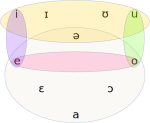
\includegraphics[height=.3\textheight]{figures/vowels_wolff.pdf}
\end{figure}

\figref{fig:wolff:4} shows the following overlaps of allophones (in terms of both impressionistic transcriptions rather than based on phonetic studies, and for ``practical'' orthography purposes), where in particular mid vowels are candidates for neutralising underlying phonemic contrasts:

\begin{itemize}
  \item{} [i, ɪ, ə, ʊ, u]    may represent non-phonemic schwa;
  \item{} [i, e]      may represent phonemic /i/;
  \item{} [u, o]      may represent phonemic /u/;
  \item{} [ə, ɛ, e, ɔ, o, a]  may represent phonemic /a/;
  \item{} [e, o]      may represent /E/ (< */a-y/, only in word-final position).
\end{itemize}

\subsection{Minimal one-vowel systems}
\label{sec:Wolff:3.5}

Comparing the PCC one-phonemic-vowel minimal system with that of Haruai of the Piawi family in Papua New Guinea, one notes at least four points of typological similarity. First, in both languages one is dealing with phonemic one-member minimal vowel systems, namely /ə/ in Haruai (according to \citet{Comrie1991} and \mbox{*/a/} in PCC). Second, [i] and [u] are the predictable syllabic variants of */y/ and */w/, respectively. Third, there is a non-phonemic/epenthetic non-low vowel, namely [ɨ] in Haruai and *ə in PCC. Fourth, mid vowels [e] and [o] tend to reflect underlying sequences vowel-glide-vowel, namely /əyə/ and /əwə/ in Haruai, which correspond to */aya/ and */awa/ in PCC. 

The situation in the Salishan language Nuxálk, also known as Bella Coola, is also typologically close. The language is described as having a minimal vowel system /i, a, u/, reminiscent of broad assumptions concerning Afroasiatic languages. According to \citet[3ff.]{Nater1984}, there is only one vowel in the language, /a/. The other vowels, [i] and [u], are claimed to be in near-complementary distribution with /j/ and /w/, respectively. 

\subsection{Outlook on Afroasiatic} 
\label{sec:Wolff:3.6}
Given the findings of the survey of Central Chadic and other similar languages, one might wonder whether there exists a correlation between minimal vowel systems, in particular those with only one or two underlying vowels, and the presence of contrastive secondary articulations of consonants which condition vowel quality (and Y-and W-prosodies, similar to those). Both such articulations and ``coloured'' vocalic allophones might first be phonetic and later phonologise adding new segmental phonemes, both vowels and consonants, to the phonemic inventories.

Chadic is the largest and possibly most diverse language family within the Afroasiatic phylum. In the light of my recent comparative research on the Central Chadic languages (\citealt{Wolff2022a, Wolffinpressb}), one could possibly expect to find that Chadic as a whole, as well as the Afroasiatic languages from other families within the phylum (Ancient Egyptian, Berber, Cushitic, Semitic, possibly Omotic), might also possess, or have possessed historically, comparable minimal vowel systems and prosodies. This, to the best of the author’s knowledge, has not (yet) been widely researched or documented. Nonetheless, there are promising leads in this direction from disparate traces in the literature.

First, there is scattered evidence from the three other branches of Chadic (West- and East-Chadic, and Masa). \citet{Schuh2002} reports the operation of morphological Y-prosody in West Chadic-A Bole and West Chadic-B Miya, Duwai, Bade, and Ngizim. \citet{Roberts2007} reports prosodies in East Chadic-A Somrai, Gabri, Kabalai, and East Chadic-B Mawa, as well as from the Masa branch (He’de). Given the heavy evidence from the Central Chadic languages, this leads \citet[139]{Roberts2009} to conclude “that the prosodies may have been characteristic of Proto-Chadic from its early days”, but have “seriously eroded” in the branches other than Central Chadic. In this regard, this would make Central Chadic the phonologically most archaic of the four branches of Chadic.

Second, one Berber language, namely Tashelhiyt, has explicitly been described along the lines of a PCC-type minimal vowel system. Indeed, Tashelhiyt and the Central Chadic languages share a number of typological features in this regard. There is, however, a methodological problem in this comparison. For Central Chadic, there is fairly robust comparative evidence regarding the diachronic evolution of these languages, while for Tashelhiyt one would be dealing just with a synchronic system of one modern language \citep{DellElmedlaoui1985}. In order to overcome this methodological hurdle, I will here confront modern Tashelhiyt (based on \citealt{Kossmann2012}: 28ff., who follows \citealt{DellElmedlaoui1985}) with two modern CC languages with minimal vertical vowel systems, namely Lamang (see \citealt{Wolff2015}) and Mandara (\citealt{Mirt1969, FluckigerWhaley1981, WolffNaumann2004}; see also \citealt{Frajzyngier2012} for a non-prosodic approach to the language). 

Tashelhiyt (Northern Berber) has a three-member vowel system /a, i, u/ plus an epenthetic central vowel [ə], the latter being considered a controversial segment, both phonetically and phonologically \citep{Kossmann2012}. The insertion of schwa is determined by the need to syllabify a sequence of consonants according to their relative sonority. The latter is built on a hierarchy that rests on the inherent sonority of segments (for Tashelhiyt: \textit{a} \textit{> i/y}, \textit{u/w} > liquids > nasals > voiced fricatives > voiceless fricatives > voiced stops > voiceless stops). As in Central Chadic languages, the high vowels [i, u] are allophones of the approximants \mbox{/y/} and /w/ rather than independent phonemes. \citet[30]{Kossmann2012} reports that the “vocalic realizations are found when the phoneme is in a syllabic position, while the semivowels are found when the phoneme is in non-syllabic position. This correctly describes most instances of \textit{y}, \textit{w}, \textit{i}, and \textit{u} in Tashelhiyt. Given a complementary distribution of the allophones [y, i] and [w, u] as a function of a syllable nucleus versus a syllable margin, the vowel system of Tashelhiyt would be reduced to a one-member system with only /a/ plus epenthetic schwa.\footnote{Actually, modern Tashelhiyt appears to have undergone a phoneme split which has created phonemic high vowels besides the semivowels /y/ and /w/ (see \citealt{Kossmann2012}: 31, based on \citealt{Boogert1997}: 247--249, 253). Such phoneme splits have been proposed for the (Central) Chadic languages in the process of vocalogenesis as well \citep{Wolff2017}.} 

This situation is nearly identical to that in Lamang (\citealt{Wolff2015}, Vol. 1: 64ff.) and other Central Chadic languages, such as Mandara of a neighbouring language group. In Lamang (\textsc{Lamang}), an apparent synchronic four-vowel system /a, i, u, E/ plus an epenthetic [ə] can be reduced, historically and by observing a complementary allophonic distribution of /y{\textasciitilde}i/ and /w{\textasciitilde}u/, to a one-vowel system with the only vowel /a/. This succeeds if one accepts a historical analysis in which word-final /E/ (with conditioned allophones [e, o]) reflects an original bi-morphemic diphthong *aY (< *a\{-y\}). This diphthong surfaces by default as [e] under an automatic palatalisation prosody, and as [o] under a labialisation prosody. Pro- and epenthetic schwa plays a sonority-based role for surface syllabification, similar to Tashelhiyt. 

Mandara’s (\textsc{Mandara}; \citealt{Mirt1969, FluckigerWhaley1981}) native words, i.e. excluding loans and phonetically long synchronic vowels, appear to have two short vowels /a, ə/. The latter has a highly intriguing synchronic allophony: apparently, /ə/ → [e] in word-final position. \citet{WolffNaumann2004} identify final [e] as a result of monophthongisation of an underlying historically bi-morphemic sequence /a-y/ and consider [ə] to be epenthetic and inserted in a sonority-based fashion. All this is parallel to neighbouring Lamang. Such a reanalysis ascribes to Mandara a minimal vowel system with only one short vowel /a/, parallel to Lamang and Tashelhiyt (Berber).\footnote{Note that this analysis for Mandara is at variance with that presented by \citet{Frajzyngier2012}, who postulates three phonemic vowels /a, i, u/ plus an epenthetic vowel and ``harmony'' processes. This reflects Frajzyngier’s preference for a non-prosodic approach to Central Chadic phonology and his disregard of the */y{\textasciitilde}i/ and */w{\textasciitilde}u/ allophony. Such an analysis was already pursued in his Gidar monograph \citep{Frajzyngier2008}, which was promptly refuted by \citet{Schuh2010}.}

This parallel in vowel system typology between Tashelhiyt (Berber) and the Chadic languages, in particular those of the Central Chadic branch, may indicate a somewhat closer relationship between Proto-Berber and Proto-Chadic (maybe a shared ``Libyco-Chadic'' node in the Afroasiatic family tree model). This link is nowadays obscured by a strong typological impact of Arabic phonology on other Berber languages. Possibly, Tashelhiyt has preserved an archaism from a very distant common past, just as the Central Chadic languages have done. This very tentative hypothesis, however, needs thorough investigation in future research (see \citealt{Wolff2022b}).

Third, as exciting as the Tashelhiyt case, there is challenging typological evidence coming from modern Semitic languages, for instance, Arabic dialects and Ethiosemitic Chaha.\footnote{These studies were pointed out to me by Cormac Anderson (p.c. 2022).} \citet{Bellem2007, Bellem2008} studied what she calls ``consonant resonance'' in Arabic dialects. Bellem’s consonant ``resonance characteristics'' and ``resonance domains'', in particular her ``resonance elements A, I, U'', stunningly resemble the ideas tentatively discussed in this paper regarding the ultimate origin of ``vocalogenesis'' and prosodies in Chadic. Namely her ``I element'' corresponds to my Y-prosody, and her ``U element'' to my W-prosody. Her ``A element'' involves some back resonance like pharyngealisation. This is parallel to tentative assumptions about the pharyngeal-approximant origins of */a/ which, however, in PCC reconstructions is no longer operational. Rather, one can postulate ∅-prosody, which, however, is no more than the absence of the other two prosodies.

\citet{Banksira2000} described the complex morphophonology of Chaha, an Ethio\-sem\-itic language belonging to the ``Gurage'' cluster, based on the analysis of a minimal /a, ə/ vowel system plus epenthetic [ɨ]. Interestingly in this context he notes:

\begin{quote}
There is no glide vs vowel contrast, so [i] and [y] represent /I/ while [u] and [w] represent /U/. In most cases, the mid peripheral vowels [o, e, ɔ, ɛ] are biphonemic, i.e. [o] is the fusion of /ə/ and /U/, [e] of /ə/ and /I/, [ɔ] of /a/ and /U/ and [ɛ] of /a/ and /I/ \citep[3]{Banksira2000}.
\end{quote}

His high ``vocoids'' /U/ and /I/ behave a lot like W- and Y-prosodies in CC languages. Not only do they account for the emergence of mid vowels, but they also affect the consonantal inventory. According to \citet[xxix\,ff.]{Banksira2000}, the consonant inventory of most Gurage languages is highly enriched by the creation of non-phonemic sounds such as the labialized labials (\textit{pʷ}, \textit{fʷ}, \textit{bʷ}, \textit{mʷ}) and palatalized velars (\textit{k’ʸ}, \textit{kʸ}, \textit{gʸ}, \textit{ç}), which are not found in Proto-Ethio-Semitic. The enrichment of the consonant system appears to relate to a simultaneous impoverishment of the vowel system. The frequency of the front vowels \textit{i}, \textit{e}, \textit{ɛ} is much lower than that of the central vowels \textit{a}, \textit{ə}, \textit{ɨ}, and the frequency of the back vowels \textit{u}, \textit{o}, \textit{ɔ} is much lower than that of the central vowels but much the same as that of front vowels. Banksira proposes the features /U/ (a phonemic element found in all back vowels) and /I/ (a phonemic element found in all front vowels), which always abandon their articulators and float to dock on preceding targets. So /U, I/ are not pronounced independently, which makes them similar to Central Chadic W- and Y-prosodies.

Arguably, in Chaha, one may not be dealing with the “impoverishment of the vowel system” \citep{Banksira2000} but with an original minimal vowel system plus, in my own terms, a prosodification of the [+high] feature shared by palatal and labiovelar (co-)articulation. Despite the differences in detail, studies like those of Bellem and Banksira open an inroad for promising comparative and typological research in a broader Afroasiatic perspective by including evidence from living Semitic languages into the comparison to the Chadic and Berber evidence. Currently, the author is not aware of any related research on Coptic, Cushitic, or Omotic languages. 

Another interesting aspect regarding modern Semitic vowel systems is a widely reported ``collapse'' of short *i and *u into schwa in many dialects of Arabic.\footnote{This may have motivated \citet[193]{Newman2006} to suggest a similar scenario for Central Chadic. In order to explain the distribution of minimal /a, ə/ vowel systems there, he suggested its origins as ``collapsed'' from a system of short and long */a, aa, i, ii, u, uu/, which he reconstructed for Proto-Chadic.}  In Arabic dialects, the resulting (sub-)systems with two short vowels /a, ə/ obviously do not mirror any archaic minimal-vowel-system situation like that reconstructed for PCC. On the contrary, they have begun to obscure the original triangular nature of a short-vowel /a, i, u/ system, which still survives in a number of Arabic dialects. According to \cite[21]{Watson2002}, in certain dialects of Arabic today, *{i} and *{u} have collapsed to schwa and are only rarely distinctive. This merger leaves these dialects with a two-short-vowel system: open /a/ versus semi-closed /ə/. For a number of other dialects, an opposition between /i/ and \mbox{/u/} exists in certain contexts, but has been reduced greatly.

As it arises from the present chapter, synchronic two-vowel systems of the /a, ə/ type in modern Afroasiatic languages may have different historical origins. On the one hand, they may represent an early stage in the unfolding of vocalogenesis (possibly from a ``vowelless'' proto-system that one might wish to equate with Proto-Afroasiatic) towards a minimal vowel system as one finds in (Central) Chadic languages. On the other hand, they may represent a much later ``collapse'' of a preceding richer vowel system, as one finds in Arabic dialects and possibly other modern Semitic languages through a general path of vowel reduction. It remains to be shown by further research whether and how the triangular short-vowel-system /a, i, u/ in Semitic links up with a still hypothetical vowelless system in Proto-Afroasiatic. In the latter, the syllabified approximants *ʕ, *y and *w might have operated almost exclusively in the vocalic space (i.e. as syllable-nuclei allophones [a, i, u]), possibly allowing also a central epenthetic vowel schwa to play a distinctive yet non-contrastive role for forming syllabic nuclei.

\section{Conclusion}
\label{sec:Wolff:4}
Minimal vowel systems, as the ones discussed in this chapter and as can now be considered characteristic for the Central Chadic languages, may be viewed as phonological rarities, but they are by no means unique in cross-linguistic perspective. 

Central to the analysis and description of such minimal vowel systems is the recognition of the complementary allophonic distribution of /y{\textasciitilde}i/ and /w{\textasciitilde}u/. In Afroasiatic including Chadic languages, the approximants /y/ and /w/ count as consonants when they form part of the ``consonantal root'', but function as vowels in the vocalic domain when their position is that of a syllable nucleus or peak. This has the effect of creating vowel systems without phonemic high vowels, which leaves low /a/ and non-low schwa (\textit{ə}), whether the latter is considered to be phonemic or not, to constitute vertical minimal vowel systems.

In Central Chadic languages, minimal vowel systems associate with a regime of prosodies, i.e. most of all palatalisation and labialisation, which create rich surface vowel inventories in terms of prosodically ``coloured'' allophones and variants, but reflect maximally two underlying vowel phonemes, /a/ and /ə/, or only one (/a/) in systems in which schwa is best considered to be a non-phonemic intrusive vowel that becomes inserted in processes of consonant syllabification.

Minimal vowel systems are not easily to discover simply by looking at synchronic descriptive data. They may require sophisticated and highly abstract phonological analysis to be conducted for the underlying representations in synchronic perspective, as well as for the reconstruction of the proto-language system in diachronic perspective. As in the case of Proto-Central Chadic, methodologically sound analyses on both sides of the Saussurean Firewall can then be considered together and thereby add a historical dimension as the following step after the abstract synchronic analyses. 

\sloppy\printbibliography[heading=subbibliography,notkeyword=this]
\end{document}
